% This is the root file of the thesis: thesis.tex

%%===================================
% \documentclass[12pt, oneside]{report}
\documentclass[12pt, twoside]{report}

\usepackage{url}
\usepackage[utf8]{inputenc} % This defines the font-encoding you prefer to use
\usepackage[pdftex]{graphicx}
\usepackage[bindingoffset=1cm,centering,includeheadfoot,margin=2cm]{geometry}

\usepackage{amsmath,amsfonts,amssymb,amsthm} % mathematical expression, symbols, fonts, and the whole theorem environment engine

\usepackage[
    citestyle=numeric-comp,
    backend=bibtex,
    bibencoding=inputenc
    ]{biblatex}
\addbibresource{refs.bib}

\usepackage{setspace}
\linespread{1.5}
\setcounter{tocdepth}{2} 
\usepackage[colorlinks=true, pdfstartview=FitV,
linkcolor=blue, citecolor=blue, urlcolor=blue]{hyperref}
\setlength{\parindent}{0pt} % No indentation between paragraphs
\setlength{\parskip}{10pt} % Space between paragraphs

% Tables
\usepackage{ltxtable}
%\usepackage{arydshln}
%\usepackage{tabu, longtable}
\usepackage{booktabs}

% Needed for code listings
\usepackage{listings}
\usepackage{color}

% Subfigure
\usepackage{subcaption}
\usepackage{import}
\usepackage{pgf}
\newcommand\inputpgf[2]{{
\let\pgfimageWithoutPath\pgfimage
\renewcommand{\pgfimage}[2][]{\pgfimageWithoutPath[##1]{#1/##2}}
\input{#1/#2}
}}
\usepackage{floatpag} % to move floatpagenr to topright

% Fussnote
\usepackage[hang]{footmisc}
\setlength{\footnotemargin}{-0.8em}

\usepackage{csquotes}
\usepackage{afterpage} % needed for empty page after front

%Pseudocode
%\usepackage[linesnumbered,german]{algorithm2e}
\usepackage[linesnumbered,english]{algorithm2e}

%%===================================
% Custom definitions
    
% Signal color
\definecolor{signalColor}{RGB}{164, 63, 114}
\newcommand\signal[1]{\textbf{\textcolor{signalColor}{#1}}}
    
% List with less space between items
\newenvironment{cList}{
\begin{itemize}
  \setlength{\itemsep}{0pt}
  \setlength{\parskip}{0pt}
  \setlength{\parsep}{0pt}
}{\end{itemize}}

% Enumeration with less space between items
\newenvironment{cEnum}{
\begin{enumerate}
  \setlength{\itemsep}{0pt}
  \setlength{\parskip}{0pt}
  \setlength{\parsep}{0pt}
}{\end{enumerate}}

% Space LoL
\let\Chapter\chapter
\def\chapter{\addtocontents{lol}{\protect\addvspace{10pt}}\Chapter}

% Code definition JSON
\definecolor{numberColor}{RGB}{24,118,129}
\newcommand\JSONnumbervaluestyle{\color{numberColor}}
\newcommand\JSONstringvaluestyle{\color{signalColor}}

\newif\ifcolonfoundonthisline

\makeatletter

\lstdefinestyle{json}{
  showstringspaces    = false,
  keywords            = {false,true},
  alsoletter          = 0123456789.,
  morestring          = [s]{"}{"},
  stringstyle         = \ifcolonfoundonthisline\JSONstringvaluestyle\fi,
  MoreSelectCharTable =%
    \lst@DefSaveDef{`:}\colon@json{\processColon@json},
  basicstyle          = \ttfamily,
  keywordstyle        = \ttfamily\bfseries
}

\lstset{
  numbers=left,
  lineskip={-1.5pt},
  captionpos=b,
  basicstyle=\footnotesize\ttfamily,
  xleftmargin=1cm,
  breaklines=true
}

\newcommand\processColon@json{%
  \colon@json%
  \ifnum\lst@mode=\lst@Pmode%
    \global\colonfoundonthislinetrue%
  \fi
}

\lst@AddToHook{Output}{%
  \ifcolonfoundonthisline%
    \ifnum\lst@mode=\lst@Pmode%
      \def\lst@thestyle{\JSONnumbervaluestyle}%
    \fi
  \fi
  \lsthk@DetectKeywords% 
}

\lst@AddToHook{EOL}%
  {\global\colonfoundonthislinefalse}

\makeatother
% End code definition JSON

% Rename listings and toc
\renewcommand{\contentsname}{Table of Contents}
\renewcommand{\lstlistlistingname}{List of Listings}

\begin{document}

%%========================================
% Frontmatter

%!TEX root = ../thesis.tex

%This is the front page
%%=========================================
\thispagestyle{empty}


\includegraphics[width=\linewidth]{fig/Logo_Header}
\mbox{}\\[1pc]
\begin{center}
    \huge{ \bfseries Using Reinforcement Learning to Size Tasks for Scientific Workflows}\\[2pc]

    \Large{Nicolas Zunker}\\
    \large{n.zunker@campus.tu-berlin.de}\\[1pc]
    \large{December 13, 2021}\\[2pc]

    BACHELOR'S THESIS\\
    Distributed and Operating Systems Chair\\
    Technische Universität Berlin
\end{center}
\vfill

Examiner 1: Prof. Dr. Odej Kao
\hfill\llap{Advisor: Jonathan Bader}\\
Examiner 2: Prof. Dr. Volker Markl

\afterpage{\null\thispagestyle{empty}\newpage}
 % This is the titlepage
\setcounter{page}{0}
\pagenumbering{Roman}
%!TEX root = ../thesis.tex

%This is the Preface
%%=========================================
\cleardoublepage
\section*{Declaration}
\addcontentsline{toc}{section}{Declaration}
I hereby declare that I have created the present work independently and by my own without illicit assistance and only utilizing the listed sources and tools.\\

Hiermit erklaare ich, dass ich die vorliegende Arbeit selbststaandig und eigenhaandig sowie ohne unerlaubte fremde Hilfe und ausschliesslich unter Verwendung der aufgefaehrten Quellen und Hilfsmittel angefertigt habe.

Die selbständige und eigenständige Anfertigung versichert an Eides statt:
\begin{center}
Berlin, den 13. Dezember 2021\\[3pc]
Nicolas Zunker
\end{center}

%!TEX root = ../thesis.tex

%This is the Acknowledgment
%%=========================================
\cleardoublepage
\addcontentsline{toc}{section}{Acknowledgment}
\section*{Acknowledgment}

I would like to thank my advisor Jonathan for his helpful advice, constructive feedback and assistance, Prof. Dr. Toussaint, Prof. Dr. habil. Kao and Prof. Dr. Zubow whose courses I enjoyed immensely and from whom I learned a lot, and my friends and family for their support.

\nocite{fan2020,learningToSchedule,scarl,toussaint}


\begin{flushright}
NZ\\[1pc]
\end{flushright}

%!TEX root = ../thesis.tex

%This is the Summary
%%=========================================
\cleardoublepage
\addcontentsline{toc}{section}{Abstract}
\section*{Abstract}

The growth of computational power and the increasing importance of digital data in scientific research has led to greater demand for computational resources  by users who aim to process large datasets. Particularly in the natural sciences it has become common for scientists to break down their computing needs into a sequence of smaller tasks, a so called workflow. These workflows can then be run on a variety of different execution platforms, depending on the users needs.

Since workflows are composed of segregated inter-dependent tasks which can run independently of each other, the individual tasks which make up a workflow can be assigned a fraction of the computational resources available to the entire execution platform, and doing so intelligently could improve efficiency and performance.

This thesis aims to investigate how reinforcement learning can be applied to the allocation of resources to individual tasks in order to choose more efficient allocations. A reinforcement learning solution will be integrated into the source code of a popular scientific workflow management system and tested with several common bioinformatic workflows. Two different approaches (Gradient Bandits and Q-learning) will be used and their performance will be compared with both that of the default resource allocations and that of an approach based on \cite{tovarjob,FeedbackBasedAllocation} which uses a feedback loop.

Ultimately the approaches presented in this thesis outperform the workflow's default configurations with regards to both memory and CPU efficiency: the q-learning approach assigned 7\% less CPU hours, 31\% less memory and was 7\% faster, whereas the gradient bandit approach assigned 42\% less CPU hours, 80\% less memory and was only 4\% slower. The feedback loop approach assigned 13\% less CPU hours, 87\% less memory and was 7\% faster and thus performed worse than the gradient bandits with regards to CPU efficiency but better in terms of memory and speed. 

%%=========================================
%\cleardoublepage
\addcontentsline{toc}{section}{Zusammenfassung}
\section*{Zusammenfassung}

Die Relevanz von digitalen Daten und die damit verbundene Analyse von grossen Datensätzen in der wissenschaftlichen Forschung wächst kontinuierlich, und der Nutzerbedarf an Rechenressourcen steigt mit. Besonders in den Naturwissenschaften ist es üblich, dass Wissenschaftler die Analyse dieser Daten in kleinere Arbeitspakete aufteilen, so genannten Tasks, und die gesamte Sequenz dieser Tasks wird als Workflow bezeichnet. Die Workflows bestehen aus verschiedenen, eigenständigen Tasks die unabhängig voneinander ausgeführt werden können, daher muss ihnen nur ein Bruchteil der Rechenressourcen des Plattforms auf dem sie ausgeführt werden zugewiesen werden.  Durch intelligente Allokationen ermöglicht dies eine größere Effizienz und Leistung der Workflows.  

Die Forschungsfrage dieser Arbeit beinhaltet wie und mit welchem Effekt Reinforcement Learning für die Allokation von Rechenressourcen zu den Tasks eines Workflows angewandt werden kann.  Hierzu werden zwei verschiedene Ansätze (Q-learning und Gradient Bandits) in den Quellcode einer Workflow Verwaltungssoftware integriert und mit fünf Bioinformatik Workflows getestet. Diese Ergebnisse werden verglichen mit der Leistung der Workflows unter normalen Konfigurationen, und einem Ansatz mit Hilfe von Rückkopplungsschleifen, der auf \cite{tovarjob,FeedbackBasedAllocation} basiert.

Die in dieser Arbeit entwickelten Ansätze zeigten eine bessere Leistung als die Workflows mit voreingestellten Allokationen, sowohl im Bezug auf die Arbeitsspeichernutzung, als auch auf die CPU Nutzung.  Der q-learning Ansatz allozierte 7\% weniger CPU Stunden, 31\% weniger Arbeitsspeicher und die Rechenleistung war 7\% schneller. Der gradient bandit Ansatz allozierte 42\% weniger CPU Stunden, 80\% weniger Arbeitsspeicher und die Rechenleistung war nur 4\% langsamer. Letztlich hat der Ansatz mit der Rückkopplungsschleife 13\% weniger CPU Stunden und 87\% weniger Arbeitsspeicher alloziert und war 7\% schneller, und damit weniger effizient mit seiner CPU Allokationen als die gradient bandits aber besser in Bezug auf Arbeitsspeicher und Geschwindigkeit.

%\newpage
%\addcontentsline{toc}{section}{Zusammenfassung}
%\section*{Zusammenfassung}

%Der Aufstieg des Internet of Things (IoT) stellt uns vor neue Herausforderungen bezueglich der Speicherung, Verarbeitung und Darstellung von Daten

\tableofcontents

\clearpage
\phantomsection
\addcontentsline{toc}{section}{\listfigurename}
\listoffigures

%\clearpage
%\phantomsection
%\addcontentsline{toc}{section}{\listtablename}
%\listoftables
%
%\clearpage
%\phantomsection
%\addcontentsline{toc}{section}{\lstlistlistingname}
%\lstlistoflistings

%%=========================================
% Mainmatter

\cleardoublepage
\setcounter{page}{0}
\pagenumbering{arabic}
%!TEX root = ../thesis.tex

\cleardoublepage
\chapter{Deterministic Multipath Backhaul Exposee - Masters Thesis}

\label{cha:introduction}

%%=========================================
\section{Motivation and Problem Description}
\label{sec:motivation}

One of the aims for the fifth generation of mobile networks (5G) and it's successors will be a greater diversification of the classes of service. As the use cases for these networks evolve, there is a greater need for quality of service (QoS) tailored to each use case. For example, in Industrial Internet of Things (IIoT) applications the bandwidth requirements are often quite low, however the requirements on latency, jitter, and reliability may be extremely stringent. Supporting these kinds of classes of service can be a challenge for mobile network operators (MNOs) and will require novel approaches to familiar problems, such as backhaul.

With more backhaul solutions becoming available (i.e. LEO satellite links, and mmWave backhaul) and adding to the existing set of options (DSL, optical fibre, DOCSIS, dedicated lines, etc.) network operators may choose to utilize more than one backhaul connection at once in order to increase the available bandwidth or to utilize the different qualities of the backhaul links. Such a situation, could then be used to achieve higher quality of service by intelligently selecting on which link to forward packets. This approach bears similarity to multihoming as well as to multi-path routing, and can take inspiration from the existing body of research in these fields which has demonstrated that QoS can be improved by using multiple paths simultaneously \cite{akella2003measurement, tao2005improving, habib2007improving, goldenberg2004optimizing, huang2008multiconstrained, akella2008performance}.


%\LTXtable{\textwidth}{tab/scenario1_sensor}

%%=========================================
\section{Goal of the Thesis}
\label{sec:goal}

\begin{figure}[h]
    \centering
        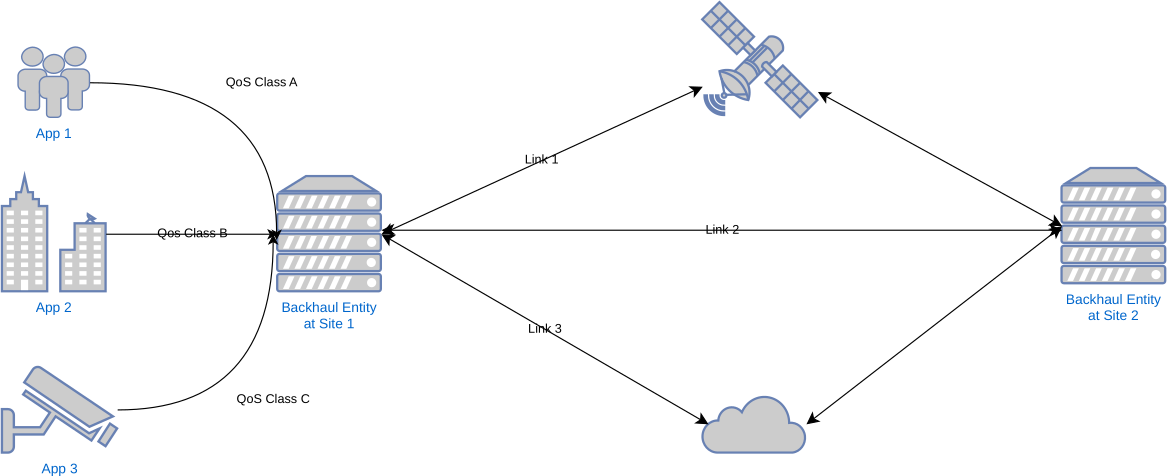
\includegraphics[width=\textwidth]{fig/use_cases.png}
        \caption{Use Case for the Backhaul Entity}
        \label{fig:use}
\end{figure}


\begin{figure}[h]
    \centering
        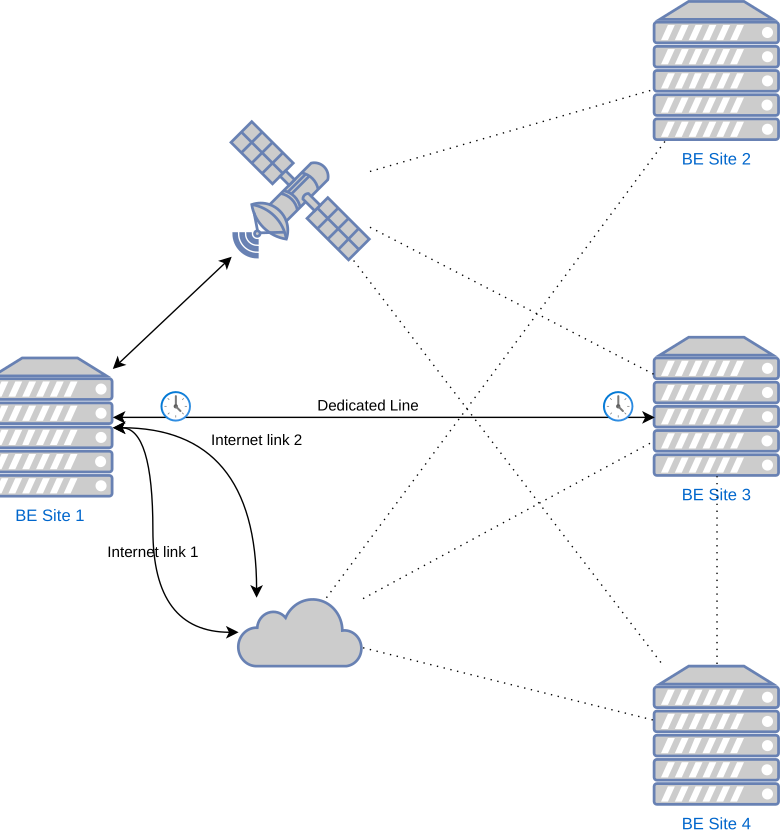
\includegraphics[width=0.75\textwidth, height=0.75\textwidth]{fig/mesh_network.png}
        \caption{Network of Backhaul Entities}
        \label{fig:mesh}
\end{figure}

The goal of this thesis is to design a backhaul entity, that can be placed at the ingress and egress point of connected networks, and which can intelligently forward packets on one or more links in order to meet specific QoS requirements. The performance of this approach will then be quantitatively analysed in experiments. Looking at figure \ref{fig:use} we can see how this is envisioned to work: A backhaul entity is deployed in 2 or more sites which have more than one egress link. Then, using the multiple links, the traffic is backhauled to the second site, while respecting it's QoS requirements. An example of how this entity could be deployed in multiple sites, interconnected in a mesh network, can be seen in figure \ref{fig:mesh}. This could allow network operators to provide more reliable quality of service for it's users, especially for important applications (e.g. between industrial sites).

%%=========================================
\section{Structure of the Thesis}
\label{sec:structure}

The planned work for the thesis will be structured as follows:

\begin{enumerate}
\item{\textit{Design}: Research existing approaches and solutions, and design an approach for reliable backhaul over multiple paths/links}
\item{\textit{Implementation}: Implement said approach in a basic testbed consisting of a traffic generator, various link emulators, measurement devices, and the backhaul entities}
\item{\textit{Evaluation}: Analyse the performance of the backhaul entity according to its ability to reduce latency, improve jitter, and provide any other QoS requirements. And compare it's performance with the performance of each individual link, as well as the performance of a round robin packet forwarding approach which utilises each link equally.}

\end{enumerate}

\begin{figure}[h]
    \centering
        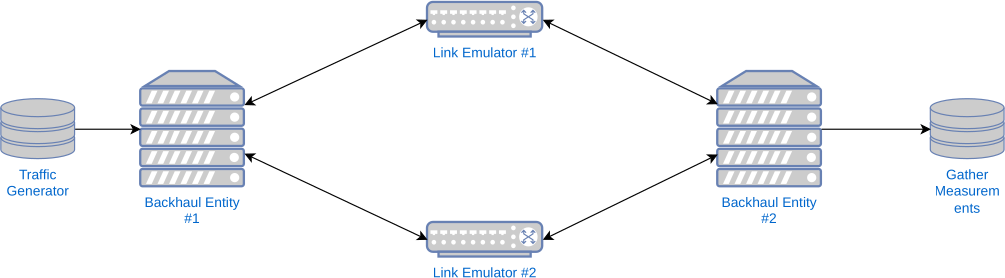
\includegraphics[width=\textwidth]{fig/testbed.png}
        \caption{Testbed Setup}
        \label{fig:testbed}
\end{figure}

The structure of the report will be a simple 5 chapter format: 1) Introduction, 2) Background and Related Work, 3) Approach, 4) Evaluation, 5) Conclusion. The approach chapter will discuss the proposed solution, and the evaluation chapter will encompass the design of the testbed and an analysis of the results.

\subsection{Timescale}

A thesis should take 6 months, or roughly 26 weeks. At present it is proposed to divide those 26 weeks into 4 equal sized chunks. The first 3 chunks will correspond to the 3 items mentioned previously in this section, the final "chunk" will be to finish writing up the report, however it is planned to do some writing during the other 3 chunks as well. In the first period - the \textit{Design} period, chapters 1 and 2 will also be worked on. After the \textit{Implementation} period is finished, chapter 3 can be written. Chapters 4 and 5 can then be written after the \textit{Evaluation} period finishes. That leaves the final chunk of time, which can be used to revise the document, as well as a buffer in case other parts of the thesis take longer to do.

The first phase of the experimental work will consist of setting up the testbed. This means installing the measurement modules as well as the link emulators. The next phase will require the implementation of the backhaul entity, as designed. The backhaul entity will require a module for collecting per-metric links, as well as the implementation of an algorithm to select the best link or links for a given flow. In the course of designing and preparing the backhaul entity there may be room for adjusting the initial plan based on what we experience during development. Next, the entity must be tested. During this phase traffic replays will be played over the testbed and evaluated. Thereafter the round robin approach and the "god routing" approach will also be evaluated. These two approaches will serve for comparison with the performance of the backhaul entity. Finally, this data must be analyzed, and the thesis can reach its conclusions, with 1 or 2 weeks buffer room for last minute revisions.


\begin{figure}
\begin{ganttchart}[expand chart=\textwidth, vgrid, hgrid]{1}{26}
  \gantttitle{Week}{26} \\
  \gantttitlelist{1,...,26}{1} \\
%  \ganttgroup{Group 1}{1}{7} \\
  \ganttbar{Literature Review}{1}{2}  \ganttbar[bar/.append style={fill=lightgray}]{}{3}{4} \\
  \ganttbar{Setup Testbed}{2}{4} \\
  \ganttbar{Implement Approach}{4}{8}] \ganttbar[bar/.append style={fill=lightgray}]{}{9}{10}  \\
  %ganttbar[bar/.append style={fill=lightgray}]{}{14}{14} \\
  \ganttbar{Metric Collection}{5}{7} \\
  \ganttbar{Link Switching Algorithm}{6}{8}\\
  \ganttbar{Adjust and Improve}{7}{9} \\
  \ganttbar{Measurements}{10}{16}  \ganttbar[bar/.append style={fill=lightgray}]{}{16}{18} \\
  \ganttbar{Round Robin}{12}{14} \\
  \ganttbar{God Routing}{14}{16}  \\
  \ganttbar{Evaluation}{18}{20}  \ganttbar[bar/.append style={fill=lightgray}]{}{21}{22} \\
  \ganttbar{Finish Writing Thesis}{21}{23}  \ganttbar[bar/.append style={fill=lightgray}]{}{24}{26} \\
  % \ganttlinkedbar{Task 2}{3}{7} \ganttnewline
 % \ganttmilestone{Milestone}{7} \ganttnewline
  \ganttlink{elem2}{elem3}
  \ganttlink{elem4}{elem8}
  \ganttlink{elem5}{elem8}  
  \ganttlink{elem6}{elem8}
  \ganttlink{elem7}{elem8}

 \ganttlink{elem9}{elem12}
 \ganttlink{elem10}{elem12}
 \ganttlink{elem11}{elem12}

\ganttlink{elem12}{elem14}

\end{ganttchart}
\caption{Gantt Chart: 01.06.23 - 01.12.23}
\end{figure}

\section{Envisioned Approach}

\subsection{Collecting Per-Link Metrics}

In order to realize such a backhaul entity, the entity needs to be able to maintain a set of metrics about the available links to aid it in choosing which links to utilize. This may not always be straightforward, and could require prediction of link quality based on previous measurements.

\subsubsection{Measurement-based Metrics}

In \cite{akella2008performance} the authors collected both passive metrics (looking at response times for outgoing packets), and active measurements (sending ICMP ping, or TCP SYN messages and measuring the response time). It is important to note that using the passive measurements enabled their multihomed approach to perform well, but when using the active measurements the performance was better. Crucially, the passive measurements worked better over larger sampling periods because it took longer to get a full overview of all the possible routes. Whereas the active sampling approach acquired it's measurements faster and was thus more effective over smaller sampling intervals.

Considering these results, it is proposed to utilize both active and passive measurements. All three metrics- packet loss, latency, and jitter- will be periodically measured in an active manner, on a site to site basis. The period over which to perform these measurements is an important design decision.

Beyond this, these metrics will also be monitored on a passive basis wherever possible. For all three metrics a response is required for each sent message, in order to measure either the time needed (for latency and jitter), or to ascertain a packet has been lost. This may only be possible for TCP SYN and SYN ACK messages, and other protocols which are guaranteed to contain certain request-response handshakes.

\subsection{Pre-configured Metrics}

Since certain links may be come with hard guarantees on packet loss, latency and jitter, this would drastically simplify the process, and thus allow us to save ourselves the measurement process for said links. Therefore the backhaul entity which will be designed, shall allow for a link to have the jitter, reliability and latency metrics pre-configured, as well as allowing them to be updated while the entity is running.

\subsection{How to Guarantee QoS}

The design of this approach is also an interesting challenge. One idea to improve jitter when backhauling across multiple links is to duplicate packets and forward them on multiple links, and have the backhaul entity on the other end buffer incoming packets and release them at a constant rate. This way in the event of a packet being lost on one link, the other link is still able to receive it and the delay caused by retransmission is avoided. The downside with this approach is that it guarantees the latency will always be that of the slowest link.

For reducing latency it would appear likely that the simplest approach may be a greedy method (as in \cite{goldenberg2004optimizing} in the online case) which always selects the lowest latency connection. However there is room for nuance here since the connection must not be overloaded and also because certain traffic may have very relaxed latency requirements but use up more bandwidth. This means monitoring the load on any one link will be important. Finally there are also more intelligent approaches, i.e. integer linear programming (used in \cite{huang2008multiconstrained} and for the offline case in \cite{goldenberg2004optimizing}) which could be used to optimally satisfy certain requirements.

The timescale over which to use a chosen link is also of interest. In \cite{habib2007improving} the time for which a link should be used is varied based on the predicted qualities of the link. These predictions are made based on past performance.

Reliability presents yet another challenge, however in a multihomed scenario it becomes easier to guarantee this via duplication, and/or forward error correction (FEC). For example if a packet flow requires 99\% reliability this can be guaranteed by duplicating packets across two links which are both only 90\% reliable. Alternatively, in such a situation, FEC could be used to pre-code the packets in order to provide the additional guarantees against packet loss and thus increase the reliability to the required level.

\subsubsection{Proposed Solution}

The solution proposed for solving this multi-constrained QoS problem is to use integer linear programming (ILP). Although ILP is NP-Complete, we can parameterize the problem by the number of outgoing links, which never needs to be more than 4, and thus brute force the solutions. The ILP constrained problem will be to select those links on which to forward packets while minimizing the overall number of links used, and making sure to satisfy the latency, jitter and reliability requirements of the given flow.

\begin{gather}
\text{Minimize } \sum_{i=1}^{P}x_i \\
\text{Where, } d(i) * x_i\le D \\
j(i) * x_i \le J \\
\text{and }1 - \prod_{i=1}^{P}{ ( 1- r(i) * x_i ) } \ge R  \\
\text{for } x_i \in \{0,1\}
\end{gather}

Here the variables $D$, $J$, and $R$ are the flow's delay, jitter, and reliability requirements, while the functions $d(i)$, $j(i)$, $r(i)$ are the predicted delay, jitter, and reliability of the link $i$ out of the $P$ total links. The predicted values will usually just be the latest measurement, as recommended in \cite{akella2008performance}, however there is room here to use more advanced metrics to predict the future link quality and thus perform preemptive path switching. The $x_i$ variable indicates whether or not link $i$ shall be used. If a solution is found, then the flow's packets will be forwarded on each link $i$ where $x_i = 1$, and if no solution can be found which satisfies these conditions then the flow is rejected because its QoS cannot be guaranteed.

\subsection{Potential Issues and Design Questions which are Still Open}

At present the idea would be to use the GTP protocol to tunnel data between any two backhaul entities, and then use the tunnel endpoint IDs (TEIDs) to differentiate between different traffic flows. In the control plane of the backhaul entity, one link would be chosen to be used for control and co-ordination messages between the two backhaul entities.

This approach could run into trouble if there is fragmentation. Some applications attempt to base their packet sizes on the most common MTU values for ethernet links (1500 bytes  minus 20 bytes for the IPv4 header and 2 bytes for UDP), and this causes a problem when the packet is tunneled because the overhead of another IP header on top of the tunnel header pushes the packet beyond the MTU and thus it has to be fragmented, which can degrade performance. In the proposed design of the testbed, there is a traffic generator at use, so this generator can be configured not to  generate packets exceeding 1450 bytes, but this issue is of practical concern for any realistic deployments.

\subsection{Evaluating Performance}

In order to evaluate the success of the proposed approach, three scenarios will be set up and investigated. Each setup will consist of two backhaul entities, and some number of emulated links going between them. The first scenario will feature 2 WAN links, a dedicated line, and a satellite connection. The second scenario will not feature the dedicated line, since it is expected that a leased line may be too obvious a choice for any of the traffic with strict QoS requirements. Finally, in order to further investigate these situations with an obviously superior candidate, the third scenario will just feature two links, a dedicated line and a WAN link.

In all of these scenarios the same traffic flows will be replayed. This traffic will contain various types of flows, with various QoS requirements. Before a new flow is started, the flow's requirements are sent to the backhaul entity and it is either accepted or rejected. During the traffic replay, the delay, jitter, and reliability will be measured.

These measurements will be performed once with the ILP approach proposed earlier and once with a simple round-robin approach for selecting links, and finally compared against an offline approach, where the optimal decision is computed with complete knowledge of the future. This offline approach will serve as the baseline for optimal performance, against which the other two approaches can be compared.


%%% include all citations

% start zotero

%\nocite{kundel_user_2022}
%\nocite{goldenberg_optimizing_nodate}
%\nocite{lange_performance_2015}
%\nocite{tarique_survey_2009}
%\nocite{tschoke_time-sensitive_2021}
%\nocite{ganichev_yamr_2010}
%\nocite{habib_improving_2007}
%\nocite{tao2005improving}
%\nocite{fanglu_guo_experiences_2004}
%\nocite{akella_measurement-based_nodate}
%\nocite{noauthor_zotero_nodate}

% end zotero...

% google translate

\nocite{tsai2006review}
\nocite{tao2005improving}
\nocite{kundel2022user}
\nocite{goldenberg2004optimizing}
\nocite{lange2015performance}
\nocite{tarique2009survey}
\nocite{tschoke2021time}
\nocite{ganichev2010yamr}
\nocite{habib2007improving}
\nocite{guo2004experiences}
\nocite{akella2003measurement}
\nocite{ergencc2021reliability}
\nocite{tao2004application}
\nocite{alwan2010multi}
\nocite{prados2021asynchronous}
\nocite{zhang2016fundamentals}
\nocite{chen2020collaborative}
\nocite{akella2008performance}
\nocite{andreoli2017mobile}
\nocite{huang2008multiconstrained}



%!TEX root = ../thesis.tex

\cleardoublepage
\chapter{Background}
\label{cha:background}


This chapter provides background information on scientific workflows and reinforcement learning and explains the functionality of these technologies within the extent to which they are related to this thesis. To begin with , in section \ref{sec:workflows} scientific workflows are discussed, then in section \ref{sec:management} the systems that manage them are introduced and finally in \ref{sec:rl} the relevant reinforcement learning approaches for this thesis are explained. 


%%=========================================
\section{Scientific Workflows}
\label{sec:workflows}

Over the last two decades computation has emerged to become an integral part of scientific research \cite{deelman},\cite{parallelization} and with the increased use of simulations and digital sensors the importance of digital data continues to rise\cite{ScientificWorkflows}. This has led to unprecedented computing power requirements in the sciences. Indeed much of the effort of scientists is now invested in the analysing and processing of the data rather than the gathering of the data, and software costs have come to dominate capital expenditures for many large-scale experiments \cite{Gray}. Some of the scientific fields which have particularly large computational needs are Biology, Astronomy, and Seismology \cite{ScientificWorkflows}. 

To handle so much data it is usually processed in a sequence of small individual steps or tasks, often using command-line tools \cite{FeedbackBasedAllocation}, in a sophisticated structure of dependencies and pipelines which can run sequentially or concurrently based on the dependencies \cite{parallelization},\cite{examining}. Since these tasks may work on the same data or a version of that data which has been processed by another task, there are of course temporal and logical dependencies between the tasks. Managing these complex interdependent structures can be quite difficult and has given rise to the concept of workflows, which are meant help model the constituent tasks and their dependencies. 

Workflows can be modelled in many different ways, ranging from simple scripting languages to graphs and mathematical models \cite{Shields}. At their core, workflows consist of four simple components: the inputs, the tasks, the dependencies between tasks, and the outputs. This can easily be modelled as a graph with vertices to represent tasks and edges to represent dependencies. An example of this can be seen in \ref{fig:dag}. 

\begin{figure}[hp]
    \centering
        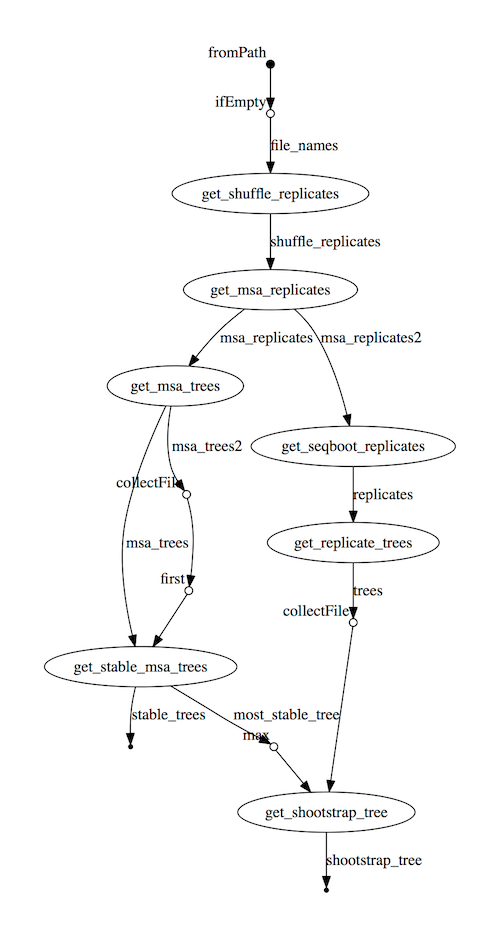
\includegraphics[width=0.45\textwidth,height=0.675\textheight]{fig/dag.png}
        \caption{nf-core/shootstrap Workflow Represented as a Digraph \cite{dag}}
        \label{fig:dag}
\end{figure}




%%=========================================
\section{Scientific Workflow Management Systems}
\label{sec:management}

The emergence of scientific workflows as a method for representing and managing these complex computations has lead to the emergence of scientific workflow mangement systems (SWMS) (or scientific workflow managers) as a means to manage the execution of scientific workflows and their constituent tasks. Today there a litany of SWMS’s available, such as Nextflow \cite{nextflow},  Kepler \cite{kepler},  Pegasus \cite{pegasus} and others.

As the resource requirements of scientific workflows can be immense \cite{ResourceProvisioning}, workflow managers must be able to interface with powerful execution platforms, which usually use resource managers such as Kubernetes \cite{kubernetes}, YARN \cite{yarn}, or other resource managers. A workflow manager will schedule a workflow’s tasks with the resource manager (this will include assigning the task a fixed amount of resources), handle failures as configured by the user, manage the communication between tasks, and if the workflow’s execution succeeds it will collect and store the results.

At this point it is important to clarify the distinct responsibilities of a workflow management system, an execution platform and a scientific workflow, with regards to the tasks. The user or creator of the workflow decides which tasks need to be executed and when they need to be executed \textbf{relative to eachother} and the SWMS will schedule tasks with the execution platform according to this design. It is the execution platform which will ultimately decide when a task will \textbf{actually} be executed on physical hardware. In this transaction it is the SWMS which is acting as the middle man. 
Beyond which tasks to execute and in which order, the user will also decide what the inputs to a task should be and the workflow manager will ensure that before the task is executed those inputs are available and that they are passed to the task. Finally with regards to resources, the user does not need to specify what the resources assigned to a task should be, the user may do so if they like, however it is not a requirement. The assignment of resources to a task is a request by the workflow management system to the execution platform, and provided the platform can fulfil these requirements then the task should be executed in an environment where it has access to as many resources as it was assigned but not more. Tasks which exceed their resource requirements will often be aborted and this will be communicated to the resource manager which will then have to decided if it should try to run the task again, continue without the task, or abort the execution of the entire workflow- all depending on the configuration of the workflow.

%%=========================================
\section{Reinforcement Learning}
\label{sec:rl}

Popularized in the seminal book by Sutton and Barto \cite{sutton_barto}, reinforcement learning can broadly be said to present a framework for a learning system or “agent” to learn the optimal policy for achieving a given goal in an uncertain environment by interacting with the problem and the environment. Most importantly it is also able to adjust this policy ``on the go'', meaning it can both learn a new policy if the challenge or the environment changes and that it can be deployed immediately into any environment without any training and it will improve as it gains experience. In this context the agent's goal is always set by a reward function. Using reinforcement learning, the agent learns to maximize this function and thus, hopefully, achieve the desire of its designers. To put it simply, reinforcement learning is a “computational approach to learning from interactions” \cite{sutton_barto}

Central to all reinforcement learning is the idea of exploration versus exploitation. Since the agent initially knows nothing about its environment it must attempt  to learn through exploration. By trying different things and receiving different rewards the agent can construct a policy that always makes the optimal choice. But in order to know what a good or an optimal choice is the learning system must also occasionally make the wrong choice so that it can learn not to make it again. Trying different things is ''exploration'' and using the knowledge gained from this to make the right choice is``exploitation''. An agent cannot simultaneously explore and exploit. This dichotomy is at the core of reinforcement learning. The agent must always make the choice between exploring more to potentially discover an even better policy and eventually yield even better rewards in the future, or using its current policy to increase its immediate rewards.

Beyond the dichotomy mentioned above, the other challenge presented to the designers of a reinforcement learning agent is the question of how to translate the overarching goals into a singular reward. A reinforcement learning agent run ad infinitum should converge to an optimal policy which maximises reward, and thus the onus is on the designer to pick a reward function which, when maximised, will help them to achieve their goals. 

\subsection{Actions, States, Policies and Rewards}
\label{subsec:agent}

For the purposes of this thesis only q-learning and gradient bandits will be discussed. In order to understand these approaches the concepts of states and actions must be introduced. An agent interacts with its environment by performing actions. These actions may have a tangible effect on the agent and the environment and the agent receives feedback about its actions. This feedback is given to the agent in the form of rewards. The agent also maintains an internal representation of itself (either independently or in relation to the environment), this representation is considered the agent’s state. An agent may change states either as a result of its own actions or as a result of changes in the external environment. A simple visual representation of these interactions can be seen in \ref{fig:agent}.

\begin{figure}[htp]
    \centering
        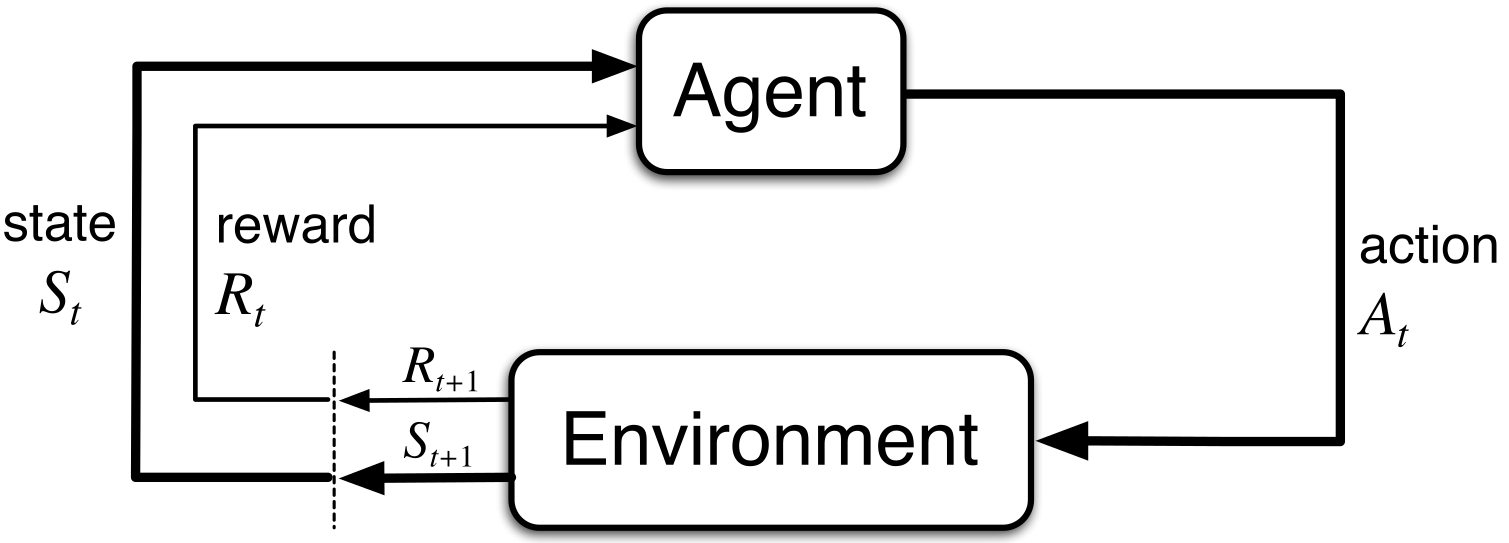
\includegraphics[width=.65\textwidth]{fig/agent.png}
        \caption{Agent Environment Interactions \cite{sutton_barto}}
        \label{fig:agent}
\end{figure}

Policies and the question of how best to evaluate them are crucial to reinforcement learning. Within the context of states, actions and rewards, a policy is simply an instruction for which actions must be taken to maximise the cumulative reward over time. Which action to take may depend on the current state or the state which the action may cause the agent to transition to. In order to achieve its goal an agent needs to develop a policy that maximizes its reward, then as the agent encounters new situations it simply follows the policy it has learned. To evaluate a given policy it must be compared to the optimal policy. For any given problem and its reward function there exists at least one policy which maximizes the reward received and could be considered optimal. At its core, reinforcement learning aims to enable the agent to continuously refine its current policy so that it approaches the optimal policy. 

\subsection{Gradient Bandits}
\label{subsection_gradient_bandits}

In this thesis two specific types of reinforcement learning are considered. First are gradient bandits. The ``Bandit Problem'' is a sequential learning problem, where each round the bandit has to decide which action to take by pulling one of $N$ levers \cite{ding_efficient}. The analogy used by Sutton and Barto is of a room with several levers, and the question of which lever to pull (the pulling of a certain lever may also be called the action). From the bandit's perspective pulling any of the levers yields a certain reward and it is the bandit's task to find a policy for pulling levers which yields the maximum reward.  Approaches to solving the bandit problem present frameworks for solving problems in which an actor repeatedly returns to an unchanging situation where there are several choices, whose consequences are not known. Applying this to the case of scientific workflow managers and the sizing of tasks one can consider the levers, or the choice, as the resource configuration. The bandit is asked repeatedly to allocate a certain amount of resources for a task (equivalent to pulling one of the levers) and must find the best policy for maximising the reward (i.e. the best “lever” or resource allocation). 

Gradient bandits solve the bandit problem by using the gradient of the reward function to learn a preference $H_t(a)$ for each of the available actions (or levers). This preference $H_t(a)$ is updated after each round $t$. Using gradient ascent the bandits take small steps in the direction of the ideal preference for each lever in order to maximize rewards. These steps are taken via stochastic gradient ascent, for which the formula is : 

\begin{equation}\label{gradient_ascent}
H_{t+1}(a) = H_t(a) + \alpha \frac{ \delta E[R_t] }  {\delta H_t(a)}
\end{equation}

This formula aims to increment the preference for an action proportional to the increment's effect on performance. The preferences influence the bandit’s probability of choosing a given action. Crucially, after choosing an action and receiving a reward, the preferences for all of the actions are updated to try and follow the gradient of the reward. In practice however the expected reward for each action is not known- if it were known the problem would be trivial and the agent could be configured to always pick the maximizing action. Instead the expected reward function and its gradient must be approximated over time. This leads to the formula for updating the preferences proposed by Sutton and Barto. For a preference $H_{t+1}(A)$ after taking action $A$ at timepoint $t$ (denoted by $A_t$) and receiving reward $R_t$ , where $\hat{R}$ is the average of all the rewards so far and $\pi_t(a_t)$ is the probability of picking action $a_t$, its preferences are updated as follows: 

\begin{align} \label{preference_update}
H_{t+1}(A_t) &= H_t(A_t) + \alpha (R_t - \hat{R}) (1 - \pi_t(A_t)) & \text{and} \\
H_{t+1}(a) &= H_t(a) - \alpha (R_t - \hat{R})\pi_t(a) & \forall a \neq A_t
\end{align}

In this formula $\alpha$ is called the step size and it is a parameter which may be a constant or a function of the timepoint $t$ but must be greater than 0. It has been proven in \cite{sutton_barto} that this formula eventually approximates the formula in \ref{gradient_ascent} for gradient ascent. 

After updating its preferences, the gradient bandit then uses these preferences to inform the probability of choosing the next action at time $t+1$. This can be done, for example, using a softmax distribution, and indeed in the rest of this thesis the softmax formula in \ref{softmax} is what is used to update gradient bandits.

\begin{equation}\label{softmax}
\pi_t(a) = \frac {e^{H_t(a)}} {\sum_{i=1}^n e^{H_t(i)}}
\end{equation}

At the start (timepoint $t = 1$) the gradient bandit’s preferences are all the same: $H_1(a_1) = 0 , \forall a$. It then chooses actions based on the probabilities determined by the preferences for each action, and updates its preferences according to \ref{preference_update} based on the reward it receives, and uses \ref{softmax} to update the probabilities, which in turn will determine the next action chosen. Through this method the gradient bandit will begin with a natural inclination to explore, and as it figures out which actions yield the greatest rewards, the probability of picking those actions will increase and the bandit will choose those actions more often, thus naturally striking a balance between exploitation and exploration. 

It should be mentioned however that this balance is dependent on the step size $\alpha$. For large values of $\alpha$ the bandit will spend less time exploring and more time exploiting. But despite this, if the nature of the rewards received for a given action begin to change, for example if an action goes from consistently receiving quite large rewards to consistently receiving poor rewards, then the formula in \ref{preference_update} will naturally begin to decrease its preference for that action and the bandit will begin exploration again- regardless of step size. This is of course one of the strengths of reinforcement learning approaches, namely that they can adapt to changes in the environment or the reward function.

Finally, some terminology- when the preference for an action has become so large that the probability of picking this action approaches 1 the gradient bandit can be said to have “converged” to this action. 

\subsection{Q-learning}

While the bandits in the previous section do not have a concept of state and must only learn about the actions available to them, stateful agents must maintain an internal state $s \in S$ and choose actions $a \in A$ which will yield new rewards and may cause them to transition to new states. The transition to a new state may also be independent of the action picked. The set of all possible states which the agent may conceivably find itself in and the set of available actions which the agent may potentially take are denoted as $S$ and $A$ respectively. Within this context of states and actions, a policy $\pi(s)$ must pick the agent’s action $a$ based on its current state $s$.

Q-learning was first proposed in \cite{watkins_dayan} and it provides a simple way for an agent to act optimally in controlled Markovian domains \cite{watkins_dayan}. An explanation of Markov domains or policy evaluation is beyond the scope of this thesis. Q-learning will therefore be explained within the context of the simplified agent-environment interface mentioned earlier (subsection \ref{subsec:agent} and figure \ref{fig:agent}). 

Q-learning is an off-policy temporal  difference control algorithm. An in depth explanation of temporal difference is also out of the scope of this thesis but a simplified explanation will come later in this section. Off-policy refers to the fact that q-learning is able to approximate the optimal action-value function independent of the policy being followed. The fundamental formula underpinning q-learning called one step q-learning:

\begin{equation}\label{eq:q-learning}
Q_{t+1}(s,a) = Q_t(s,a) + \alpha \times (r + \gamma \times max_{\hat{a}}(Q_t(\hat{s},\hat{a})) - Q_t(s,a) )\\
\end{equation}

In this formula the function $Q_t(s,a)$ is a state-action-value function. It reflects the value (which is based on both historic rewards up to timepoint $t$ and the expected future rewards) of taking action $a$ in state $s$. When an agent takes action $a$ it will receive reward $r$ and transition to state $\hat{s}$. After this the agent must update its $Q_t$ function for $s$ and $a$ to $Q_{t+1}$. If the old value function for $s$ and $a$ was $Q_t(s,a)$ then the update to this function is the difference between the old valuation and the reward plus the discounted expected value of the new state. The expected value of the new state is $Q_t(\hat{s},\hat{a})$ where $\hat{a}$ is the action which maximises $Q_t(\hat(s),a)$ and $\gamma \in [0,1]$ is the discount.

\begin{equation}\label{eq:TD}
(r + \gamma \times max_{\hat{a}}(Q_t(\hat{s},\hat{a})) - Q_t(s,a)\\
\end{equation}

This is called the temporal difference. It reflects the difference between the current approximation of the value function ($Q_t(s,a)$) and the optimal value function ($r + \gamma \times Q_t(\hat{s},\hat{a})$). If the current approximation is too optimistic then \ref{eq:TD} will be negative and on the other hand if $Q_t$ is too pessimistic or too small then the temporal difference will be positive. Using the temporal difference, $Q_t$ is then adjusted by the temporal difference multiplied with the step size $\alpha$ to yield $Q_{t+1}$. This is what equation \ref{eq:q-learning} shows. All that is required for this iterative process to converge to the optimal value function is that all $s$,$a$ pairs continue to be updated \cite{sutton_barto}.

Using a value function built from equation \ref{eq:q-learning} an agent can approximate an optimal policy by simply using a greedy approach and always picking the action $a$ which maximises $Q(s,a)$, when it is in state $s$ (and then updating its value function according to \ref{eq:q-learning}). By building on this the epsilon greedy q-learning algorithm can be constructed. The pseudocode for this algorithm can be seen below.
\begin{algorithm}[h]
Initialise $Q(s,a) = 0$ , $\forall (s,a)$\\
Initialise start state $s$\\
\While{\textbf{True}}{
        \eIf{$random < \epsilon$}{choose action $a$ randomly}{choose action $a = max_a (Q(s,a))$}
        Take action $a$, receive reward $r$, transition to state $\hat{s}$\\
        Update $Q$: $Q_{new}(s,a) = Q(s,a) + \alpha \times (r + \gamma \times max_{\hat{a}}(Q(\hat{s},\hat{a})) - Q(s,a) )$\\
}
\caption{Epsilon Greedy Q-learning Pseudocode}
\label{alg:q-learning}
\end{algorithm}

This algorithm introduces random exploration with a probability $\epsilon$ and follows the q-learning algorithm the rest of the time. With sufficient exploration and an epsilon that eventually decreases to zero this algorithm should approximate an optimal value function and can then follow an optimal policy by greedily selecting the actions which maximise the $Q$ function it learned. This is the algorithm which will be used by all q-learning agents implemented in this thesis. A final note- since the requirement for convergence to the optimal value function is that all pairs are visited, during early runs whenever the q-learning agent encounters a situation with an action it has never chosen before, it must choose this action. Only if all the available actions have been tried at least once can it use the greedy approach of selecting the maximising action.

Similar to subsection \ref{subsection_gradient_bandits} the q-learning agent also has a step size parameter $\alpha$ and it also has to balance exploration against exploitation. However for the q-learning agent its exploration can be heavily influenced by the $\epsilon$ parameter whereas the gradient bandit’s exploration is implicitly tied to its preferences.


%!TEX root = ../thesis.tex

\cleardoublepage
\chapter{Related Work}
\label{cha:related_work}

This chapter discusses other works in related areas and considers the nuances of their approaches and how they differ from the one presented in this thesis. First there will be a discussion of select pieces of literature which use reinforcement learning approaches for allocating resources in \ref{sec:rl_allocation}, and then three papers related specifically to resource management within the context of scientific workflows will be considered in \ref{sec:workflow_allocation_papers}. All of the papers mentioned here served as important references and inspiration for this thesis. 

%%=========================================

\section{Using Reinforcement Learning to Allocate Resources}
 \label{sec:rl_allocation}
 
SmartYARN \cite{smartYarn} applies a q-learning approach to balance resource usage optimization against application performance. The need to balance reducing costs by using less resources against the need to increase runtime by using more resources is one of the central considerations for any client of a cloud computing platform. In this paper the researchers used the performance of the application under a certain resource configuration as the state-space, while the action-space was made up of just 5 actions: increasing or decreasing one unit of CPU or memory, or keeping the previous allocation. In the end the researchers found that the agent was able to achieve 98\% of the optimal cost reduction and generally performed at the optimal level, finding the optimal allocation the vast majority of the time.

This paper served as the inspiration for the q-learning approach used in this paper and is also one of the few works discussed in this section which considers the central issue of cost versus performance when assigning resources. One significant difference however is that SmartYARN only seeks to optimise individual jobs which do not depend on each other, whereas for scientific workflows the jobs (or tasks) are part of a larger workflow and depend on each other and may need to wait for other tasks to complete before they are ready to be executed.

\cite{vconf} tackled a similar problem: configuring the resource allocations of virtual machine's (VM's) using reinforcement learning. Their approach modelled the problem as a continuing discounted Markov Decision Process and solved it with q-learning. The states were always a triple of CPU Time credits (used for scheduling cpu time), virtual cpu's (vCPU's), and memory. The agent's available actions were increasing, decreasing or leaving the allocations, with only one resource allowed to be changed per action. As a reward the ratio of the achieved throughput to a reference throughput was used. The key trick used by the researchers was to use model based reinforcement learning. By modelling states the agent is able to simulate or predict the reward it can expect from previously unseen action-state pairs, whereas the classic q-learning approach used in this paper requires the agent to experiment with each action-state pair. This means the model based agent is able to learn much faster and can enter its exploitation phase earlier than the static agent which must explore the action-state space for a long time, especially when there are large state spaces. Ultimately however the researchers found that the static agent performed quite well and achieved high levels of throughput in its own regard, although the model-based approach consistently outperformed the static one. 

This paper's problem and its solution to it are again quite similar to those of this thesis but there is a significant difference because it schedules the resources of virtual machines as opposed to the resources of individual jobs. Another difference is the use of model based reinforcement learning to limit the time spent exploring the state action space to approximate a value function and spend more time exploiting this function to achieve better results. 

Finally there is the DeepRM \cite{DeepRM} paper on resource management using deep reinforcement learning. Here the researchers used a policy gradient reinforcement learning algorithm combined with a neural network. The state-space consisted of the resources of the cluster and the resource requirements of arriving jobs, encoded as so called "images" which could be fed into the neural network. The actions available to the agent were simply to choose a job and allocate resources to it. In order to speed up the process the agent was given the option to schedule up to $M$ jobs in a row, thus enabling it to leap forward by as many as $M$ timesteps instead of always progressing by a single timestep. The reward given to the agent was the negative average slowdown. In the end the researchers' approach outperformed both the shortest job first metric and a very strong, heuristic based algorithm called Tetris \cite{tetris}. A key reason that the agent was able to achieve this increased performance was that it learned a policy to maximize the number of small jobs it completed. While the approach taken in the paper was still better with large jobs it was significantly better with small jobs because the network learned to always keep a small amount of resources available to quickly service any small jobs which might arrive, whereas the other approaches inevitably scheduled all the available resources so that small jobs also had to wait.

The similarities here are relatively few since this paper also had to concern itself with the decision of which job to allocate and when, whereas this thesis only considered how much of a given resource to allocate to a task. Beyond that there is also the fact that a neural network was employed and the decision to use the resources of the system to model the state of the agent. Though this is an idea which could be interesting as a topic of further research if one were to expand on this thesis. What is most interesting however is the policy that the neural network was able to learn. It was able to maximise throughput by always reserving a small amount of resources for small tasks which re-occur often. This kind of advanced strategy is something that could be built into an algorithm but the ability of a reinforcement learning agent to learn such a strategy shows their potential for impressive results within the field of scheduling and resource assignment.

\section{Resource Allocations in Scientific Workflows}
\label{sec:workflow_allocation_papers}

 In \cite{tarema} the researchers used cluster profiling to build node groups with similar performance profiles and map a task to a node group based on historical performance data. A 3 step system is used. In step 1 the cluster profiles are built based on microbenchmarks and hardware analysis tools. Then in step 2 the tasks are labelled in the SWMS based on their monitoring data. Finally, in the third step dynamic task-resource allocation is performed based on the information from the previous steps. Using this approach the authors were able to achieve a mean reduction of job runtimes of 19.8\% compared to popular schedulers, and a reduction of 4.54\% compared to the shortest-job-fastest-node (SJFN) heuristic. 

This target of that paper is of course much more similar to that of this thesis than any of the previously mentioned papers, however the obvious difference is that this thesis approaches task resource assignment with a reinforcement learning approach. One other similarity is that this paper used the exact same SWMS (nextflow) as this thesis. Beyond that it would be an interesting area of research to try and combine the topic of that paper with the topic of this thesis and try and apply reinforcement learning to task resource assignment amongst node groups with similar performance profiles.

Next, in \cite{FeedbackBasedAllocation} a feedback based resource allocation system for the scheduling of scientific workflows is designed. Their approach uses an online feedback-loop to improve resource usage predictions and thus more accurately allocate resources to the constituent tasks of a scientific workflow. Tasks within scientific workflows were assigned memory based on percentile or linear regression predictors. One such percentile predictor, called PC50, worked by using the median memory usage of a task as its prediction. This approach was significantly outperformed by the \textit{LR mean} approach which was a linear regression predictor that predicted memory usage based on a linear regression that relates a task’s input data to its memory usage. This prediction is then offset by the standard deviation between the predicted and the true peak memory usage.

This paper addresses a very similar problem to that of this thesis but attempts to use linear regression to predict memory usage whereas this paper is focused on using reinforcement learning. Of course it also does not attempt to predict CPU usage or assign CPUs to tasks. The PC50 approach and \textit{LR mean} approaches ultimately served as inspiration for the feedback loop approach with which the agents in this thesis are compared. The feedback loop approach used in this thesis takes the PC50 predictor and adds an offset based on standard deviation, much like \textit{LR mean}, to try and predict memory usage. 

Finally there is \cite{tovarjob} which presents a job sizing strategy for tasks in scientific workflows. The researchers used equations based on integrals over the resource usage to either minimise waste or maximise throughput. When gathering training data they assigned tasks the maximum allowable value for all of their resources. This was repeated until the task’s resource usage statistics began to converge. Then they used their analytical solution to assign resources and if the task failed or was killed it was retried again with the maximum available resources. Ultimately an increase in throughput of between 10 and 400 was achieved.

The approach in this paper also served as inspiration for the feedback loop approach used here. The idea to assign the maximum resources available and observe a task’s performance is an interesting strategy for determining how to size a task. It could be considered an alternative form of exploration to that in reinforcement learning because it determines a task's resource requirements based on the task's usage when the maximum possible amount of resources are available as oppposed to exploring different allocations. It is critical to note that an assumption is made that a task’s resource usage does not depend on the available resources. Lastly unlike in \cite{FeedbackBasedAllocation}, which only considers memory, \cite{tovarjob} looks at CPUs and disk space and how to assign these resources to tasks within scientific workflows.

\section{Points of Interest from these Works}
\label{sec:takeaways}

All of the papers discussed in section \ref{sec:rl_allocation} managed to utilize reinforcement learning in an administrative fashion to improve the performance of jobs in their respective computing environments. A common theme among the papers was to limit the action space to increasing, decreasing or keeping the current allocation or resources and storing the current allocation as the agent’s state. This approach is also used here for the q-learning agent. The majority of the papers also utilized neural networks and it is also worth noting that most of them used runtime in their reward functions. 

In section \ref{sec:workflow_allocation_papers} the topic of resource management in scientific workflows was looked at and the papers mentioned all tended to use more analytical approaches. Indeed there is relatively limited literature regarding combining machine learning and scientific workflow management. A consistent theme in the papers about sizing tasks in scientific workflows is the idea that a task’s resource requirements are relatively static and can be learned over time using linear regression or profiling.  One topic which is not really addressed in these papers is the relationship between resource assignment and performance, because assigning a task more resources (which may be less efficient) can speed up performance. This is an important topic in this thesis and the papers \cite{FeedbackBasedAllocation} and \cite{tovarjob} do not mention runtime, while \cite{tarema} does mention it but does not deal with task sizing. In this thesis the effect of task sizing on workflow performance is an delicate tradeoff which must be balanced correctly to both reduce resource wastage and maintain reasonable runtimes and improve (or at least not harm) workflow performance.

The papers \cite{FeedbackBasedAllocation,tovarjob}in section \ref{sec:workflow_allocation_papers} both served as direct inspiration for the feedback loop approach in this thesis which is compared with the reinforcement learning agents. The approach functions by combining the training process from \cite{tovarjob} with the \textit{LR mean} allocation scheme from \cite{FeedbackBasedAllocation}.


%!TEX root = ../thesis.tex

\cleardoublepage
\chapter{Approach}
\label{cha:approach}


This chapter covers how a solution was integrated into a scientific workflow manager, as well as the specific parameters and reward functions of the reinforcement learning agents. In section \ref{sec:integration} the software architecture of the approach and its integration with the nextflow source code will be discussed, and then in \ref{sec:gradient_bandits} and \ref{sec:q_agent} respectively the details of the gradient bandit and the q-learning agents will be considered. 

%%=========================================
\section{Integrating a Solution into a Workflow Manager}
\label{sec:integration}

Nextflow \cite{nextflow} is a robust scientific workflow management system written primarily in groovy. It supports various execution platforms and has a large variety of tools to help users analyse the performance of their workflows. Nextflow is free open source software and for this thesis a fork of the 20.12.0 version was used \footnote{https://git.tu-berlin.de/zunkernicolas/nextflow-extension}. In order to integrate a reinforcement learning approach with the nextflow source code a simple structure was designed which externalised the storage of data from previous tasks and workflows so that when a task needed to be scheduled the reinforcement learning agent could retrieve historical data about the task from a database to inform its decision. The structure can be seen in the following figure.

\begin{figure}[ht]
    \centering
        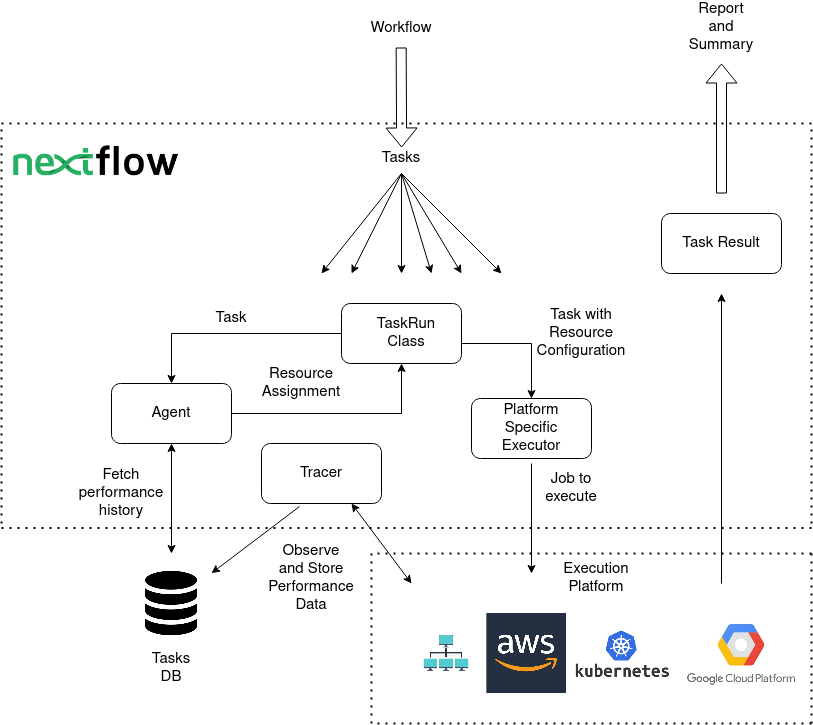
\includegraphics[width=0.8\textwidth]{fig/implementation_diagram.png}
        \caption{High Level Design: Integration of a Reinforcement-Learning Agent into Nextflow}
        \label{fig:implementation}
\end{figure}

Although the code for the reinforcement learning agents is logically a part of nextflow, when discussing the above design they will be referenced separately. The interaction between nextflow, the agents, and the external actors (the user, the database and the execution platform) is as follows. First, before a task is ready to be scheduled it is sent to a reinforcement-learning agent specific to that task, for the purposes of this thesis that was either a q-learning agent or a gradient bandit. Next, the task’s agent would then retrieve historical performance data and any other relevant data (i.e. what state the agent was last in) from the database. This database is external to nextflow and the creation and management of this database is not performed by nextflow or the agent which only use the database to save or read data beyond a workflow’s lifetime. Then, using the data, the agent selects a new resource allocation for the task and overwrites the task’s default configuration. After this, nextflow uses its custom executor for the given execution platform to prepare the task and pass it on to that platform. The task is then executed on the platform. It is important to note that the execution platform will also have its own system for managing, scheduling and executing jobs and processes. As the task is executed nextflow’s tracer module will gather performance data, i.e. peak CPU usage and peak RSS \footnote{https://www.nextflow.io/docs/}. Finally, once the task is finished all of this data is stored in the database for the agent to use the next time the task comes. It is important to note that there is one agent for each unique task. These agents are called whenever their task needs to be executed and they use the database to receive rewards for their previous actions.

Now that the structure of the agent’s environment has been explained and the relationship between collecting data and assigning a task resources is clear, it is time to delve into the specific approaches tried.

\section{Gradient Bandits}
\label{sec:gradient_bandits}

In the course of this thesis gradient bandits were used to allocate both CPUs and memory. The way they did this will be explained here.

\subsection{CPU Bandit}
\label{sub:cpu_bandit}

\subsubsection{Design}
\label{subsub:bandit1_design}

The CPU Bandit, as it was nicknamed, had a very simple set of actions to choose from which were based on the number of CPUs available to the system. The bandit then learned how many CPUs to allocate to its task. Its reward was a very straightforward function:

\begin{equation}
\label{bandit1_reward}
reward = -t\times(1+cpus - cpu\_usage/100)
\end{equation}


In this equation $cpu\_usage$ is a value in percent of the number of single core CPUs used by the task. If a task were assigned 4 CPUs and only effectively used two of them then $cpu\_usage$ would be $200$\%. $cpus$ is the number of CPUs assigned to the task and $t$ is how long the task took to run. Put in other words this equation punishes the agent with a negative reward equal to the amount of time it ran plus the unused CPU time (execution time multiplied by the number of unused CPUs). The idea is to provide an incentive for the agent to try to minimise the amount of time where any of the allocated CPU’s are not being used, and by punishing it with the amount of time that the task ran for, the agent is also encouraged to try to reduce the amount of time taken for the task to complete. This also means that, should a task have 100\% usage then its penalty is not 0 but is just the execution time. The reason for including time in the reward function is that if the agent has no concept of time it will always allocate the least amount of resources possible, since that is guaranteed to minimise the amount of resources wasted, and ultimately the tasks and their workflows would all be incredibly slow. 

\subsubsection{Picking the Right Step Size}
\label{subsub:const_stepsize}
The most pressing issue encountered with the CPU bandit approach was related to the step size. The initial step size $\alpha$ was $0.1$, which would be an appropriate step size for a bounded reward function with a mean reward that is around 10 or is known to have a standard deviation less than that (these values are based on the example given in \cite{sutton_barto} where they use a step size of 0.1 for a reward function with a statistical mean of 4). However the reward function used in \ref{bandit1_reward} has the bounds [ $-time \times (cpus+1)$ , $-time$ ] and as such is unbounded, since $time$ can be arbitrarily large and the standard deviation which was observed for the rewards was also too large. Therefore whenever tasks had a runtime $> 10$ seconds, $\alpha$ was too large. 

The danger in using a constant step size which is too large for the reward function is that when the bandit receives a reward which is considerably larger than the previous average the “step” taken in the direction of that action will also be too large and the bandits preferences will be updated such that the given action is always preferred and no other actions are tried any more. This causes the bandit to cease exploration too early. This effect was a common problem for tasks which took longer than 20 seconds to complete and was especially pronounced for tasks with runtimes of 100 seconds and more.  For these tasks the inherent volatility of the reward function relative to a step size of 0.1 meant that the bandits were converging very early and often had not explored the other actions at all. To provide a concrete example: if a bandit’s third allocation of CPUs received a reward of -150 and the first two allocations had had an average reward of -200, then for a step size of 0.1 the preference for the new allocation would increase by approximately $50\times0.1=5$. Now because of the exponential nature of the soft max distribution function used on the preferences, the probability of picking that action would increase by a large amount and then the bandit is in danger of converging to that allocation without any more exploration. This is best demonstrated graphically, as can be seen in figures \ref{fig:sub1} and \ref{fig:sub2}.

\begin{figure}[ht]
\centering
\begin{subfigure}{.5\textwidth}
  %\centering
  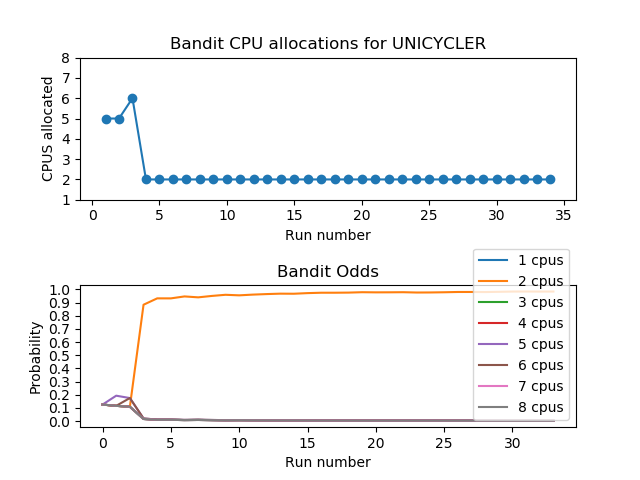
\includegraphics[width=\textwidth,height=\textwidth]{fig/old_UNICYCLER.png}
  \caption{Bandit 1}
  \label{fig:sub1}
\end{subfigure}%
\begin{subfigure}{.5\textwidth}
 % \centering
  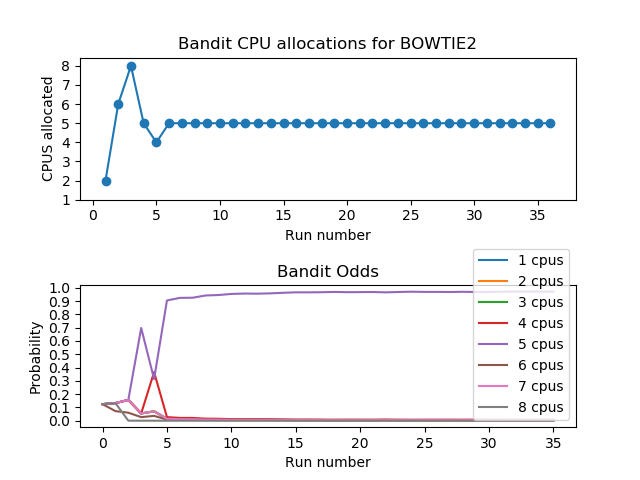
\includegraphics[width=\textwidth,height=\textwidth]{fig/old_BOWTIE2.png}
  \caption{Bandit 2}
  \label{fig:sub2}
\end{subfigure}
\caption{Example of Two Bandits Converging Too Fast}
%\label{fig:old_bandits}
\end{figure}

These figures show two gradient bandits which were exhibiting the behaviour described above. Each figure is made up of 2 graphs which display the action chosen by the bandit in the top graph and the probabilities for all of the actions in the bottom graph. As can be seen in the two examples, after receiving a relatively large reward, the agent’s probability of choosing a given action rises far too quickly and no other actions are attempted thereafter. This is occurring because the step taken by the bandit in the direction of a single action’s preference is too large and the resulting probability of choosing that action grows so much that no other actions are explored any more. 

The solution to this problem is to adjust the step size so that it is not a constant value but is instead a function which uses the average time that it usually takes the task to complete. This way tasks which have longer average runtimes are given smaller step sizes. The new value for $\alpha$ is thus $1/avg(time)$.

\begin{figure}[ht]
\centering
\begin{subfigure}{.5\textwidth}
  %\centering
  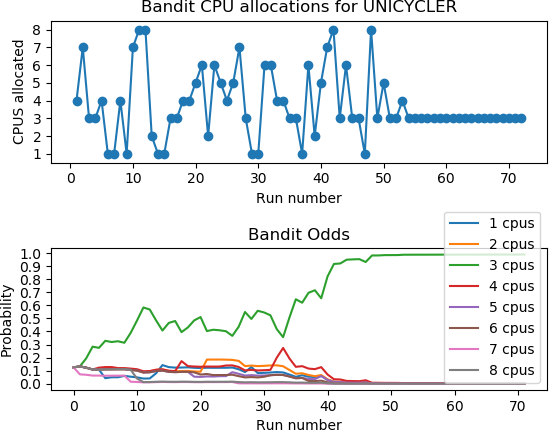
\includegraphics[width=\textwidth,height=\textwidth]{fig/UNICYCLER.png}
  \caption{Bandit 1}
  \label{fig:sub3}
\end{subfigure}%
\begin{subfigure}{.5\textwidth}
 % \centering
  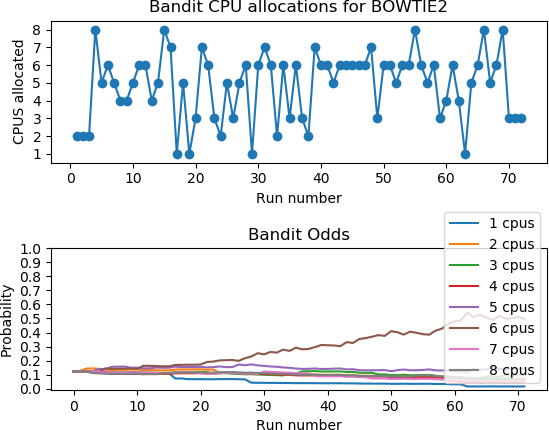
\includegraphics[width=\textwidth,height=\textwidth]{fig/BOWTIE2.png}
  \caption{Bandit 2}
  \label{fig:sub4}
\end{subfigure}
\caption{Bandits with a Step Size Based on Their Historical Average Execution Time}
\label{fig:fixed_bandits}
\end{figure}

The next two figures \ref{fig:sub3}, \ref{fig:sub4} show the same two tasks and their bandits but with the new step size. As can be seen the exploration phase is considerably longer and many different CPU allocations (actions) are tried before settling on one. Specifically in the case of the \textit{UNICYCLER} task’s bandit we can see that although allocating 3 CPUs seems to develop a strong preference early on (perhaps because it performed abnormally well once or perhaps because it genuinely is the best performing allocation) it does not become so preferred as to be dominant until much later and until that point the bandit continued to try other options.

It should be noted that these changes mean that for optimal performance of the bandits there should already be some historical data available about the task’s and their runtimes. It is not a necessity because over time the bandit can gather this data itself, but it is preferable.

\subsection{Memory Bandit}
\label{sub:mem_bandit}
The other gradient bandit approach used for assigning resources to tasks was called the memory bandit and its available actions were memory assignments. Beyond the obvious, the memory bandit was different from the CPU bandit in two respects. Firstly, the amount of memory available is several order of magnitudes larger than the amount of cpus. Thus, in order to limit the number of available actions to a manageable amount, the original amount of memory assigned to the task $m$ (in the default configuration) had to be split up into $n$ chunk,s each of size $c=m/n$. The bandit is then presented $a$ actions, each of which assigns $a\times c$ amounts of memory to the task. $a$ can be chosen as $1.5 \times n$ to give a good balance between considering allocations that are larger and smaller than the default configuration, however since it is known in advance that user estimates are usually quite poor one could also choose $a < n$ to encourage memory efficiency. In addition to this, by choosing larger or smaller $n$ values the size of the memory chunks can be adjusted. Secondly, and this is the biggest difference between the two bandits, a task which is assigned too little memory and overuses it will be killed. This means that there must be a special penalty for such cases.

The reward function used for the memory bandit, after assigning $memory$ bytes of memory is as follows:

\[ reward = 
\begin{cases}
   % \frac{x^2-x}{x},& \text{if } x\geq 1\\
    -2\times memory/c,& \text{if the task ran out of memory}\\
    -1 \times unused\_chunks              & \text{otherwise}
\end{cases}
\]

Where $unused\_chunks = (memory - peak\_rss) / c$ and $peak\_rss$ is the peak resident set size (RSS), in bytes, of the task during its execution.

An obvious alternative for this function is to simply use the memory usage: $reward = peak\_rss/mem$, and $\alpha = 0.01$ since the reward function’s range is [0,100]. However during testing this was found to be too small for tasks which have a low memory footprint. For example a task which uses 1\% of the assigned memory when assigned $n$ chunks, and thus receives a reward of 1\%, will only yield a maximum reward of $n$\% for the optimal allocation of just one memory chunk and for such small differences a gradient bandit will struggle to recognize the superior choice, even though it should be obvious. This is especially damaging to performance because these low usage tasks are precisely the ones where memory efficiency can be optimized the most and as such the reward function was changed to one which penalises the agent for the amount of unused memory. Of course to avoid the problem the CPU bandit had with its step size, the amount of unused memory in bytes could not be used and therefore the number of unused memory chunks was used instead. To return to the example of a task with 1\% usage that task’s rewards would now be $-n$ at worst and $-1$ at best, which makes it much easier for the bandit to determine good allocations. Finally in the case where a task has been killed the penalty is equal to double the number of memory chunks assigned because the agent must (at the very least) assign the same amount of memory again or must assign even more memory.

The actual implementation of the memory bandit is slightly adjusted so that whenever a task fails with one memory allocation and is retried with a new one, the new allocation must be greater than the previous one. If the bandit does pick a smaller allocation then it is ignored and the new allocation is either doubled or the default configuration for that task is used (if double the new allocation is also less than the failed allocation). This prevents the workflow from being broken off if a given task fails too many times due to repeated poor allocations.

Finally, to return to a discussion of step size similar to that in \ref{subsub:const_stepsize}, the memory bandit can be assigned a constant step size $\alpha = 1/n$. This is is because for $n$ memory chunks, the bandits reward function is bounded by [$-n$, 0]. 


\section{Q-learning Agent}
\label{sec:q_agent}

Similar to the approach with the gradient bandits, there was one q-learning agent per unique task. The q-learning agent’s state was always the current allocation of CPU and memory for the given task, and as its set of actions it could choose between incrementing or decrementing the amount of CPUs or memory, or it could do nothing. To limit the state space the maximum and minimum number of CPUs and memory as well as the amount by which they were incremented or decremented was based on the default allocation given to the task by the developers of the workflow (provided they did not exceed the resources of the execution platform). When the task was scheduled by the agent for the first time it would start in the default configuration’s state. Just like the memory bandit in section \ref{sub:mem_bandit} the possible memory states of the reinforcement learning agent are also chunks of memory. 

For the q-learning agent a different reward function was used than for the CPU bandit, primarily because it also had to incorporate memory but also as part of an attempt to experiment with different reward functions and approaches. 

\begin{equation}
\label{q_agent_1_reward}
r = -max(0.1,unused\_cpus) \times (t/avg\_t) \times (mem\times (1 - max(0.75,mem\_use)))
\end{equation}

Here the $mem$ variable refers to the memory allocated to the process and $mem\_use$ is the value of of the peak RSS of the task divided by the memory assigned to it. $avg\_t$ is a constant value which is determined at runtime based on the historical average execution time for the task. Lastly, $unused\_cpus = cpus - cpu\_usage/100$ where $cpus$ and $cpu\_usage$ are the same as in \ref{bandit1_reward}. 

Since division by the task’s average time is incorporated into the reward function it did not need to be incorporated into the step size as with the gradient bandit (see \ref{subsub:const_stepsize}) and the issues associated with that were avoided. This function is effectively a product of the number of unused CPUs, the slow-down factor and the amount of unused memory. However there are some slight modifications. The $max$ function is used to set an artificial floor for the penalty incurred by the unused CPUs and unused memory. Tasks which use more than 90\% of the available CPUs are given the same reward as tasks which use exactly 90\% in an attempt to prevent the agent from deciding to assign each task 1 CPU in order to minimise the number of unused CPUs. Additionally the floor for unused memory is capped at 25\% in a similar manner. This is done to discourage the agent from allocating too little memory because tasks which use too much memory will of course be killed and have to start over, which can have a detrimental effect on performance. This reward function is of course negated in order to turn it into a penalty function so that the agent will seek to minimise its penalty by minimising the number of unused CPUs, the slowdown and the amount of unused memory.

The q-learning agent also has 3 other parameters- the step size $\alpha$, epsilon $\epsilon$ and the discount $\gamma$. Step size was set to 0.1 and the discount was 1.0. Epsilon is adjusted over time- at first it is 0.5, to encourage exploration, then after 50 runs it is decreased to 0.25 and after 100 runs it is 0.1 to discourage exploration but leave room for the bandit to still occasionally try other actions and visit different states.

\subsubsection{Exploring the State-Action Space}
\label{subsub:states}

It should be noted here that unlike the gradient bandits from before, which had to decide from $c$ or $n$ number of actions for the CPU and memory bandits respectively, the q-learning agent must learn the value function for $(c-2)*((m-2)*a + 2*(a-1)) + 2*((m-2)*(a-1) + 2*(a-2))$ state-action combinations. Here $c$ is the number of possible CPU states, $m$ is the number of possible memory states and $a=5$ is the number of possible actions. Now since the q-learning algorithm from \ref{alg:q-learning} needs to try each action in every state combination at least once, and explores with probability $\epsilon$ then for arbitrary examples of $c=4$ and $m=3$ it will take, at the very least, 46 different runs just to have tried every action in every state once. This shows how much more complex the q-learning approach is than the gradient bandit approaches. Ultimately however the theoretical benefit posed by q-learning is that when the agent learns, for example, not to increment the amount of CPUs when in state $s$ (where $s$ is also the number of CPUs currently allocated), the agent is thus also learning to avoid all states/allocations $\{s_c \in S$ $|$ $s_c > s\}$ which allocate more CPUs than $s$. While this seems trivial, the gradient bandit is unable to see such connections and cannot tell that a task which has low CPU usage for $s$ CPUs can be expected to have even lower usage for $s_c > s$ CPUs. 



%!TEX root = ../thesis.tex

\cleardoublepage
\chapter{Evaluation}
\label{cha:evaluation}

This chapter reviews how the approach from the previous chapter was tested, and discusses the observed results. This chapter will explain the setup of the testbed, as well as the motivation behind the types of tests which were performed. Finally a discussion of the results and their origins will take place.


\section{Approach to Evaluating Performance}

In order to evaluate the success of the proposed approach a multipath scenario with four links will be emulated and investigated. Each test will consist of two WAN connectors, and the four emulated links going between them. The characteristics of the links will be changed during the tests, each time with respect to different properties: latency, packet loss, and jitter. The evaluations will be performed on a testbed consisted of four seperate host servers. Two of these servers will act as the originating and terminating WAN Connectors. One server will generate and measure traffic, in between the two WAn Connectors, a server will act as the link emulator. This architecture is shown in figure \ref{fig:testbed}

\begin{figure}[h]
    \centering
        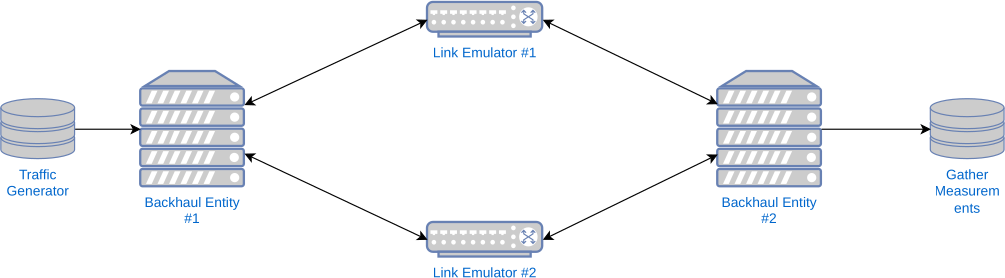
\includegraphics[width=0.66\textwidth]{fig/testbed.png}
        \caption{Testbed Setup}
        \label{fig:testbed}
\end{figure}

In figure \ref{fig:testbed}, the links between the servers are 10 GB ethernet cables. The hosts are connected as is shown. In the "traffic generator and measurer" two linux namespaces are used to separate the traffic generation and the measurement. The packets generated in one namespace are routed via the ethernet connection to the next host (the terminating or "edge" WAN Connector), because of the linux namespace they are not aware that their destination is technically the same host. The packets are then are backhauled by the WAN Connector over the emulated links in the next host, and via the terminating WAN Connector, back to the original host, but now in the "measurer" namespace.

The link emulation is done using the tc subsystem. First a root Heirarchical Token Bucket qdisc is established on the "downlink" and "uplink" interfaces (the ethernet cables between the WAN Connectors). In this case, the link emulation is performed before the outoing packet is queued on the ethernet cable, so that is also where the qdisc is placed. Secondly, the qdisc is given children classes, one class per link. This allows one to establish bandwidth caps for each emulated interface. Within these HTB classes the root qdisc is a netem qdisc. These allow the installation of link characteristics such as latency, packet loss, and jitter.

%In all of these scenarios the same traffic flows will be replayed. This traffic will contain different types of flows, with different QoS requirements. Before a new flow is started, the flow's requirements are sent to the WAN connector and it is either accepted or rejected. During the traffic replay, the delay, jitter, and reliability will be measured.

%All of these tests can be performed on the same testbed which will be set up as is shown in Figure \ref{fig:testbed}. The testbed architecture features a traffic generator, two WAN connectors, with a link emulator between them, and a measurement module to analyze performance. In practice the traffic generator and the test bench will be co-located on the same machine. The link emulator, and the WAN connectors are separate hosts, all interconnected over ethernet. The link emulation is done using the linux kernel's traffic control subsytem (TC). TC offers a network emulator (netem) queuing discipline (qdisc), which is able to emulate various link characteristics including delay, jitter, packet loss and packet re-ordering. Furthermore by combining the netem qdisc with a rate limiter, such as the Heirarchical Token Bucket (HTB) qdisc, a link can have its bandwidth limited. This allows one to emulate links with different latency, reliability and jitter, and with different maximum bandwidths.

In order to make the emulation more realistic, the netem qdiscs will periodically be adjusted, this allows one to degrade or improve links over time, for example by increasing the latency or packet loss in frequent intervals, up to a large value. It also more closely mimics the real-life behavior of WAN connections, which do experience changes in their characteristics over time.

For the purposes of evaluating the WAN connector, three series of experiments will be performed to isolate and investigate it's link switching capabilities. First, purely latency based link selection will be investigated- a flow will be defined with specific latency requirements and then the emulated links will have their latency repeatedly changed. The same will be done once with packet loss and with jitter. In each of these scenarios the other two parameters will be held constant, so that the WAN Connector can be judged based on its ability to meet one of the latency, jitter, or packet loss requirements, without the other two requirements interfering. In order to simulate realistic scenarios these experiments will also be repeated once with background traffic which aims to saturate the link's capabilities.

The data for the emulation used in all of these scenarios was obtained using the Satellite Constellation Network Emulator (SCNE) \footnote{https://connectivity.esa.int/projects/scne} from the European Space Agency. The default scenario is 24 hours long and consists of 288 satellites, 10 gateways (GW), and 50 user terminals (UT). The reason this data is used is because LEO satellite links are expected to be the most common type of backhaul link for geographically distributed 5G Campus Network deployments. Furthermore, since LEO satellite connections are exceptionally more volatile than "regular" links \cite{deutschmann2022broadband} \cite{ma2023network}. By choosing to emulate more volatile links in the testbed, the WAN Connector experiences a more difficult test, and one can be assured that the real life performance in "normal" scenarios, is highly unlikely to be worse.

Since the WAN Connector is defined to work on at most four outgoing links, each investigated scenario will feature four links. These links will all be based on data from the SCNE emulation.

\subsection{Accuracy of the Emulation}

To make sure that the testbed emulation also matches the values from the SCNE, a brief comparison was done, where the testbed's latencies were compared with those recorded in the SCNE. 

Figure \ref{fig:sim_vs_em} shows the comparison between the data observed in the testbed, and the SCNE. The testbed data in the graphic is measured by the packet flows running over the individual links. The emulation data comes from the values recorded during withh the SCNE. Since the testbed data is collected at a rate of 100 packets per second, but runs at 10 times the speed of the SCNE emulation, there are 10 times as many data points. This explains why the testbed data appears blurrier.

\begin{figure}
  \centering
  \begin{tabular}{@{}c@{}}
    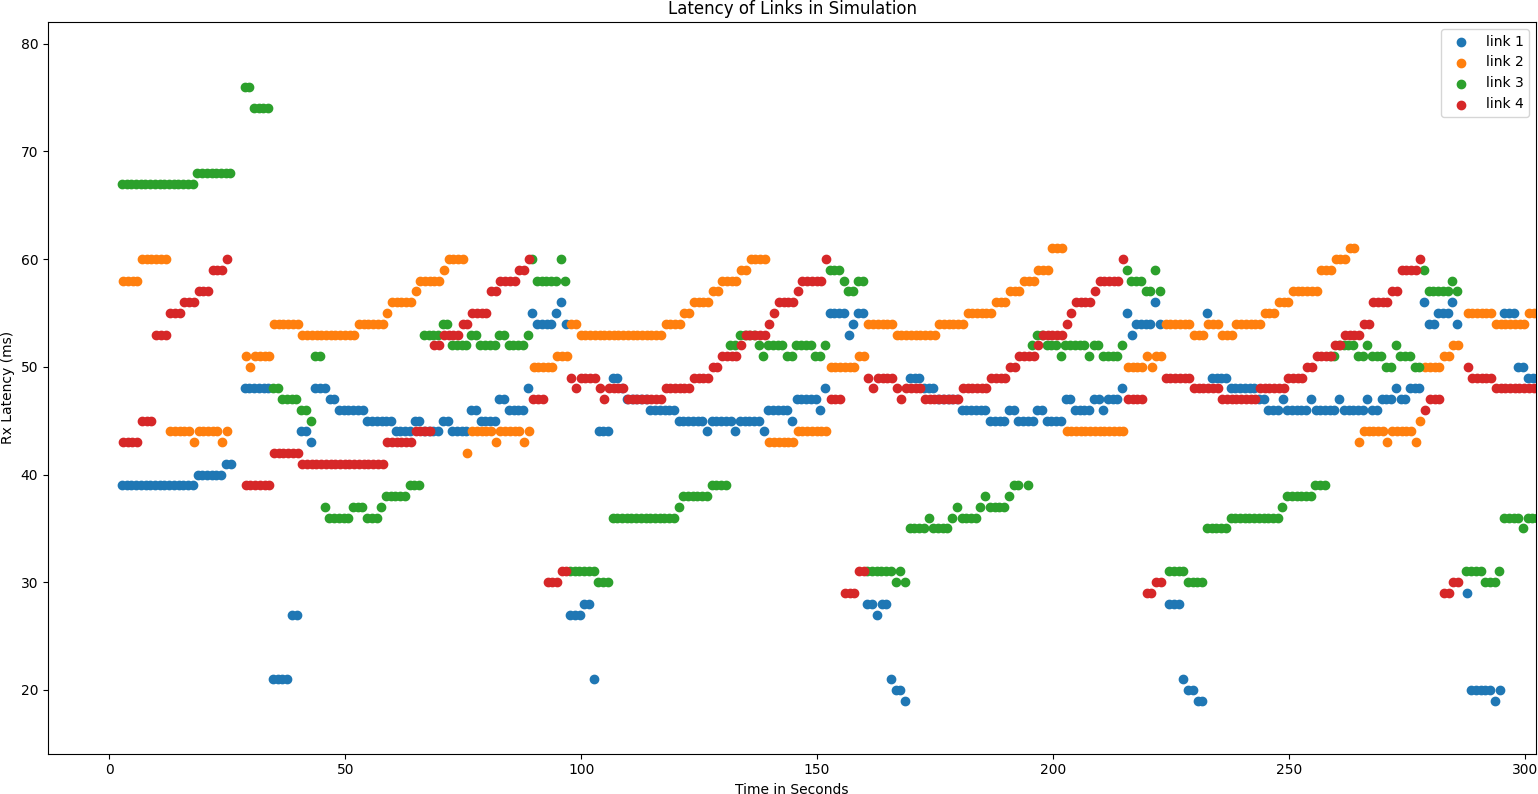
\includegraphics[width=\linewidth]{fig/simulated_latencies.png} \\[\abovecaptionskip]
    \small (a) Latencies Recorded in SCNE
  \end{tabular}

  \vspace{\floatsep}

  \begin{tabular}{@{}c@{}}
    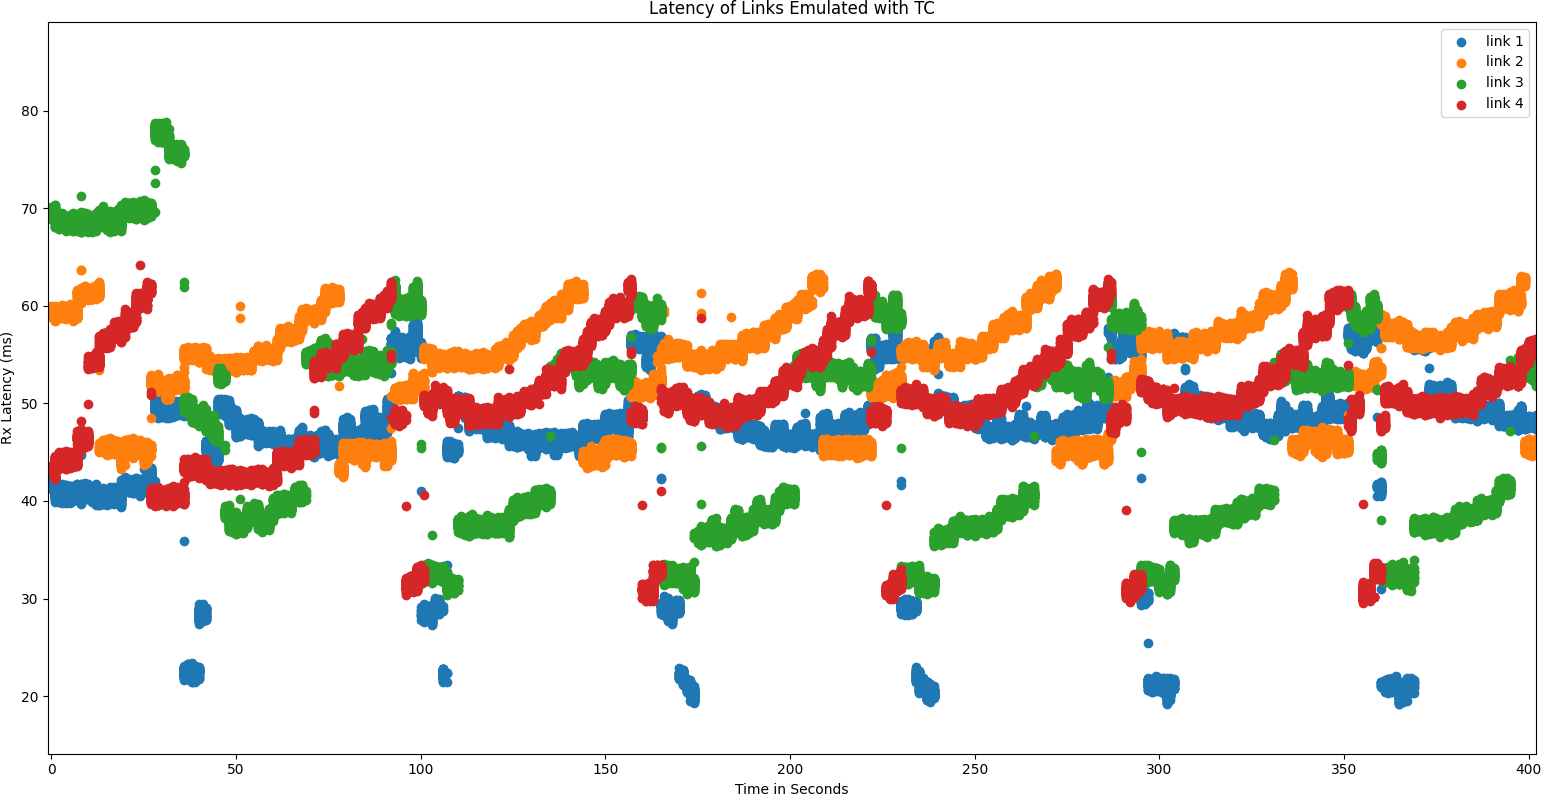
\includegraphics[width=\linewidth]{fig/emulated_latencies.png} \\[\abovecaptionskip]
    \small (b) Emulated Latencies Measured in the Testbed
  \end{tabular}

  \caption{Comparison of the Emulators Latencies and the Testbed}\label{fig:sim_vs_em}
\end{figure}

As can be seen in the figure \ref{fis:sim_vs_em}, the latencies recorded on the testbed closely match those from the SCNE, which it was seeking to replicate.

\section{Latency Based Path Switching}

First is the scenario investigating latency. During the emulation, the simulation data is used to adjust the tc netem qdisc on the "link emulator" machine periodically. Because the SCNE simulator provides latency data over a 24 hour period, in 10 second intervals, the simulation data is "sped up". That is the emulation is changed each second, based on the next datapoint from the simulation. This means the 24 hour window can be run over a 2 hours test. Since real links are usually steadier and less volatile than the sped up emulation one can expect results in a real situation to be better.

In the experiment 100 packets are sent per second across each link, as well as 100 packets per second from the traffic generator, through the WAN Connector. This is done to have a comparison between the performance of the WAN Connector and the baseline performance level, which would be the best performing link. In any scenario the minimum acceptable performance of a path switching application would be to provide a better performance than the best single link. Otherwise it would be better to just select the best link, and not use the application at all.


\subsection{Performance Compared to Single Links}

For the experiment a flow is defined in the WAN Connector with a minimum round trip time (RTT) of 56 milliseconds. This value is chosen because it is the mean of the mean values of the latencies of the four links from the emulation. For the evaluation of the latency based path switching a single flow matching the definition stored in the WAN Connector is backhauled through the WAN Connector at a rate of 100 packets per second. In order to serve as a comparison, identical 100 packet per second flows are sent across the four other links. Finally their latencies are compared, and the latencies measured by the four links are used to calculate the Oracle approach.

The graphics \ref{fig:latency_cdf1} and \ref{fig:latency_cdf1_super_zoomed_in} show a cumulative distribution of the different latencies experienced by the packet flows running over the individual links and the WAN Connector, as well as the performance of the Oracle approach. The Oracle results are purely theoretical. For each packet, it is able to select the best link to forward on, based on that links future characteristics. This approach is calculated by comparing each packet sent by the WAN Connector with the latency that packet \textit{would} experience on any of the other links, and if the latency of the WAN Connector's link would be greater than the minimum value (56 ms), selecting a different link (if one exits) with a lower latency. Since it always picks an optimal path, the Oracle approach provides an upper bound on the best possible performance. In practice it is not possible because it has knowledge of the future, but nonetheless it acts as a very valuable comparison.

\begin{figure}[h]
    \centering
        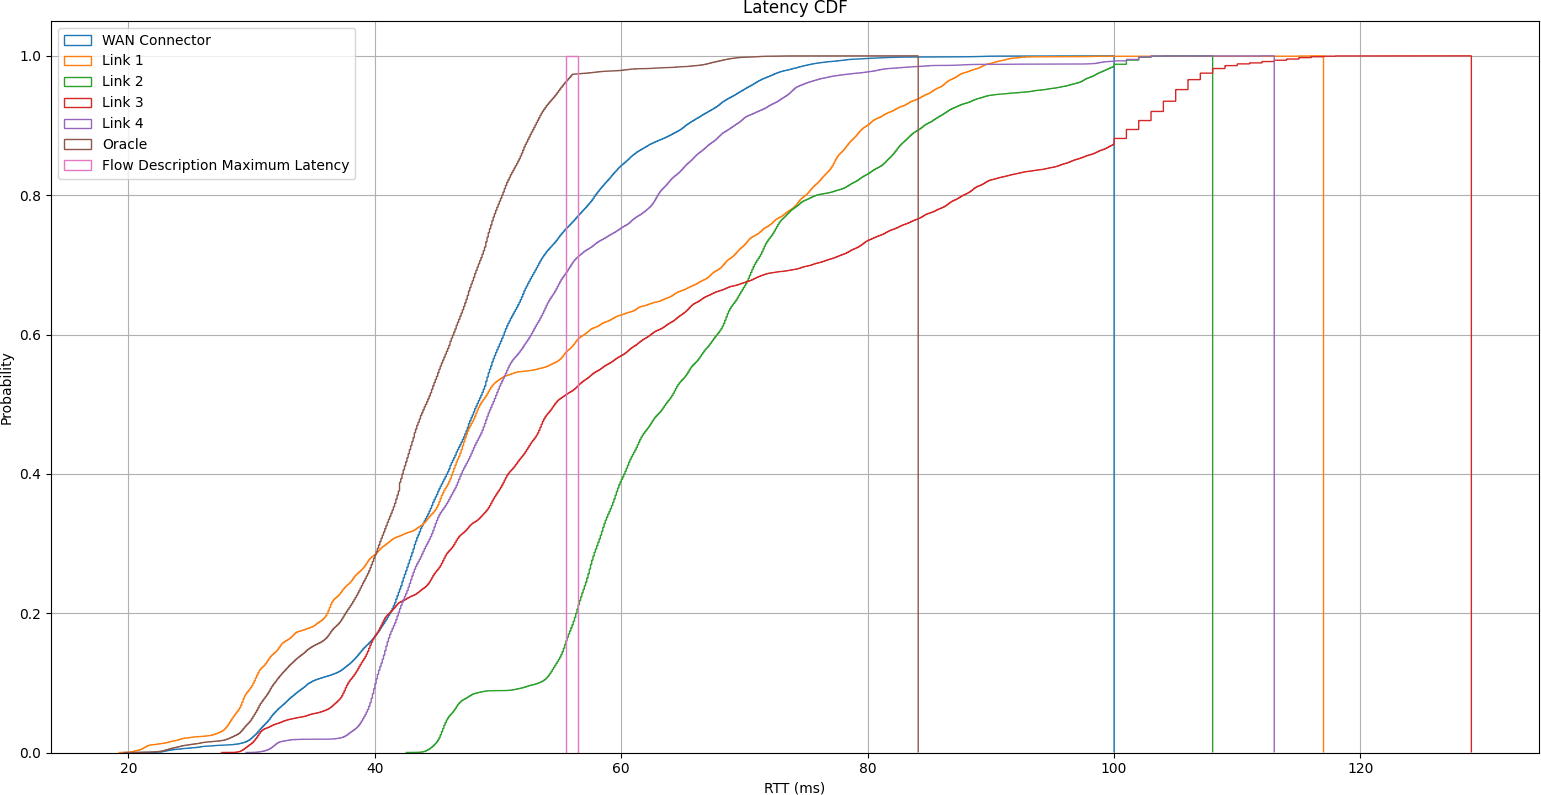
\includegraphics[height=0.8\textwidth,width=\textwidth]{fig/latency_cdf1.png}
        \caption{Cumulative Distribution of the Latencies}
        \label{fig:latency_cdf1}
\end{figure}

\begin{figure}[h]
    \centering
        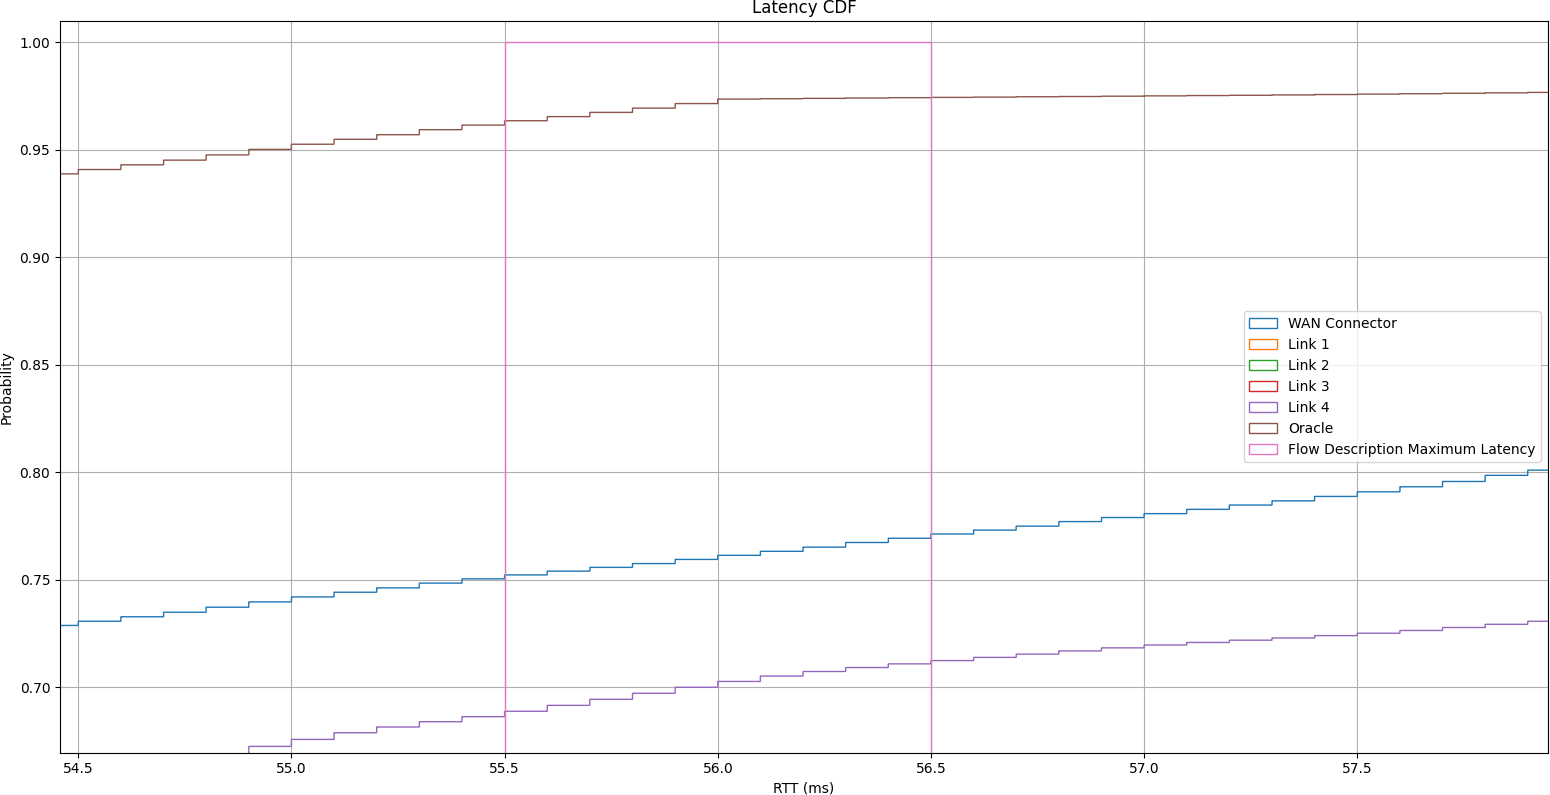
\includegraphics[height=0.66\textwidth,width=\textwidth]{fig/latency_cdf1_super_zoomed_in.png}
        \caption{Closeup of the Latency CDF}
        \label{fig:latency_cdf1_super_zoomed_in}
\end{figure}

The CDF shown in figure \ref{fig:latency_cdf1} and zoomed in on in figure \ref{fig:latency_cdf1_super_zoomed_in} tracks the probability that the flow experiences a latency less than or equal to the latency value on the y axis. The pink bar labelled "Flow Description Maximum Latency" is set at 56 milliseconds and represents latency bound for the flow being measured, which was communicated to the WAN Connector.


The results in the figures show that the WAN Connector is able to achieve a superior performance to any of the individual links on their own. This was the baseline requirement and it is important that it is able to achieve this. However the performance does not significantly improve on the next best link, which is is able to achieve the maximum allowed latency 72\% of the time, while the WAN Connector does so 77.5\% of the time. The Oracle approach shows that in theory one could, at best, have maintained the minimum latency required by the flow in 95\% of the cases. This means the WAN Connector's performance is only 80\% optimal.


\subsection{Latency Performance Under Load and the Importance of Traffic Shaping}

During this experiment, the same 100 packet per second flow from before is repeated, but background traffic is added. An iperf3 test is run across the WAN Connector at the same time as the latency critical flow, and the background traffic is given the same latency requirements, so that the WAN Connector always schedules both flows to the same link. This ensures that whatever link is being used will be saturated. Latency performance during congestion and close to congested scenarios is a crucial element of a deterministic backhaul solution. The WAN Connector's control plane only makes decision about which link to forward on- it does not perform load balancing or prioritization. The data plane does not do this either, it implements a purely First In First Out (FIFO) approach to packet queuing. This is done because the burden of implementing an appropriate packet shaper, in addition to the other multipath calculations, is too significant for the purposes of this thesis, and because very powerful traffic shaping implementations, which are easy to integrate into this solution, already exist.

\begin{figure}[h]
    \centering
        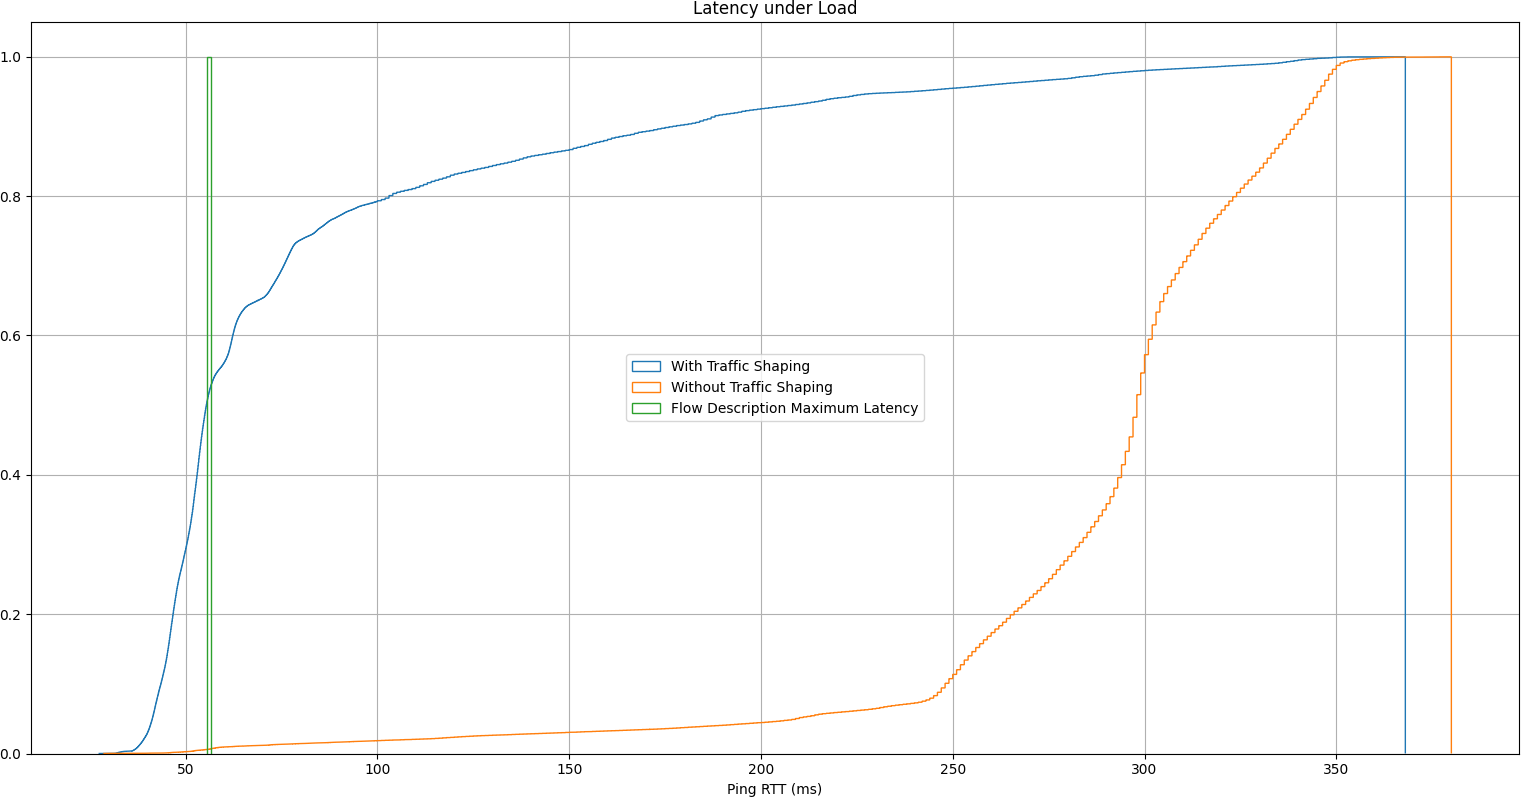
\includegraphics[height=0.66\textwidth,width=\textwidth]{fig/rrul_cdf.png}
        \caption{Latency with Background Traffic}
        \label{fig:rrul_cdf}
\end{figure}

The figure \ref{fig:rrul_cdf} neatly demonstrates why traffic shaping is an essential element of any deterministic network. In the case in which there is no traffic shaper the latency critical flow experiences significant additional latency due to the network being overloaded. The TCP algorithm fills the link's capacity, and the latency critical packets spend too much time buffering and arrive late. It should be noted that the WAN Connector's performance with the traffic shaper is worse than in the previous scenario, where there was no background traffic, and only 50\% of the packets are under the required latency of the critical flow. However the approach without the traffic shaping is at just 1\%.

\section{Reliability Based Path Switching}

In the next scenario, to analyze the ability of the WAN Connector to achieve the required reliability of a given flow, the same test flows from before are run over the WAN Connector and the four outgoing links. However this time instead of varying the latency, the packet loss ratio of the link is changed. The SCNE emulation's data is used for the testbed once again. However since the emulation does not provide packet loss on a per second basis, the latencies of all the different links in the simulation are used. For the emulation, these 51 values are looped over in 10 second increments. Each link is given a shuffled set of these 51 values. This means that the cumulative value of the packet loss experienced by all of the links is the same (2\%), but the instantaneous values will differ. To appropriately analyze this scenario the flow being backhauled over the WAN Connector is given a reliability threshold of 0.1\% this is because in this scenario, where the existing links all provide an average of 2\% reliability, it becomes necessary to duplicate at some points, in order to achieve the required reliability. Afterward, the experiment is repeated under load, like in the latency scenario, where the test flows across the links themselves are not run, and a second iperf3 flow is run across the WAN Connector in order to saturate the link. Like before, this second flow is given the exact same requirements as the test flow, in order to ensure that they are always running across the same link.

 The results of this experiment are shown in figure \ref{fig:loss_bars1}. The packet loss recorded by each of the flows over the period of the experiment is plotted in a bar graph, as well as the theoretical packet loss which would have been experienced by the Oracle approach.

\begin{figure}[h]
    \centering
        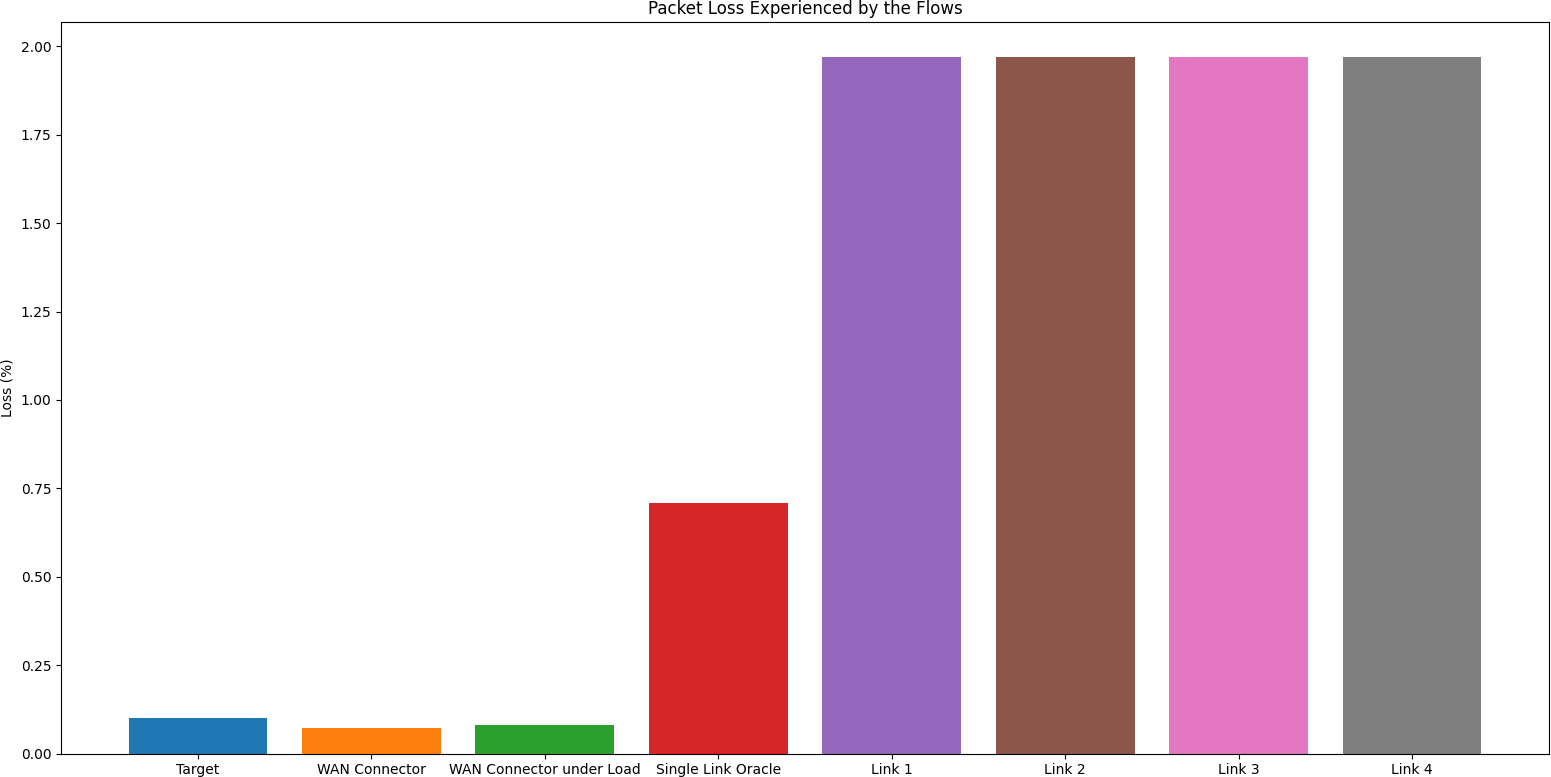
\includegraphics[height=0.66\textwidth,width=\textwidth]{fig/loss_bars1.png}
        \caption{Reliability}
        \label{fig:loss_bars1}
\end{figure}

For the analysis of the performance this time the Oracle approach is defined as choosing, before forwarding any packet, the link with the lowest packet loss ratio. But, crucially, the Oracle is not allowed to duplicate flows across different links. This explains why in figure \ref{fig:loss_bars1} the Oracle is outperformed by the WAN Connector. Indeed, as the graphic shows, it is not possible to achieve the critical flow's required reliability with any of the available links, nor with the Oracle approach. But the WAN Connector is able to achieve it. This speaks to the potency of the flow duplication approach, which is made possible in the optimization equation used to decided on which flows to forward.

\subsection{Impact on Throughput}


\begin{figure}[h]
    \centering
        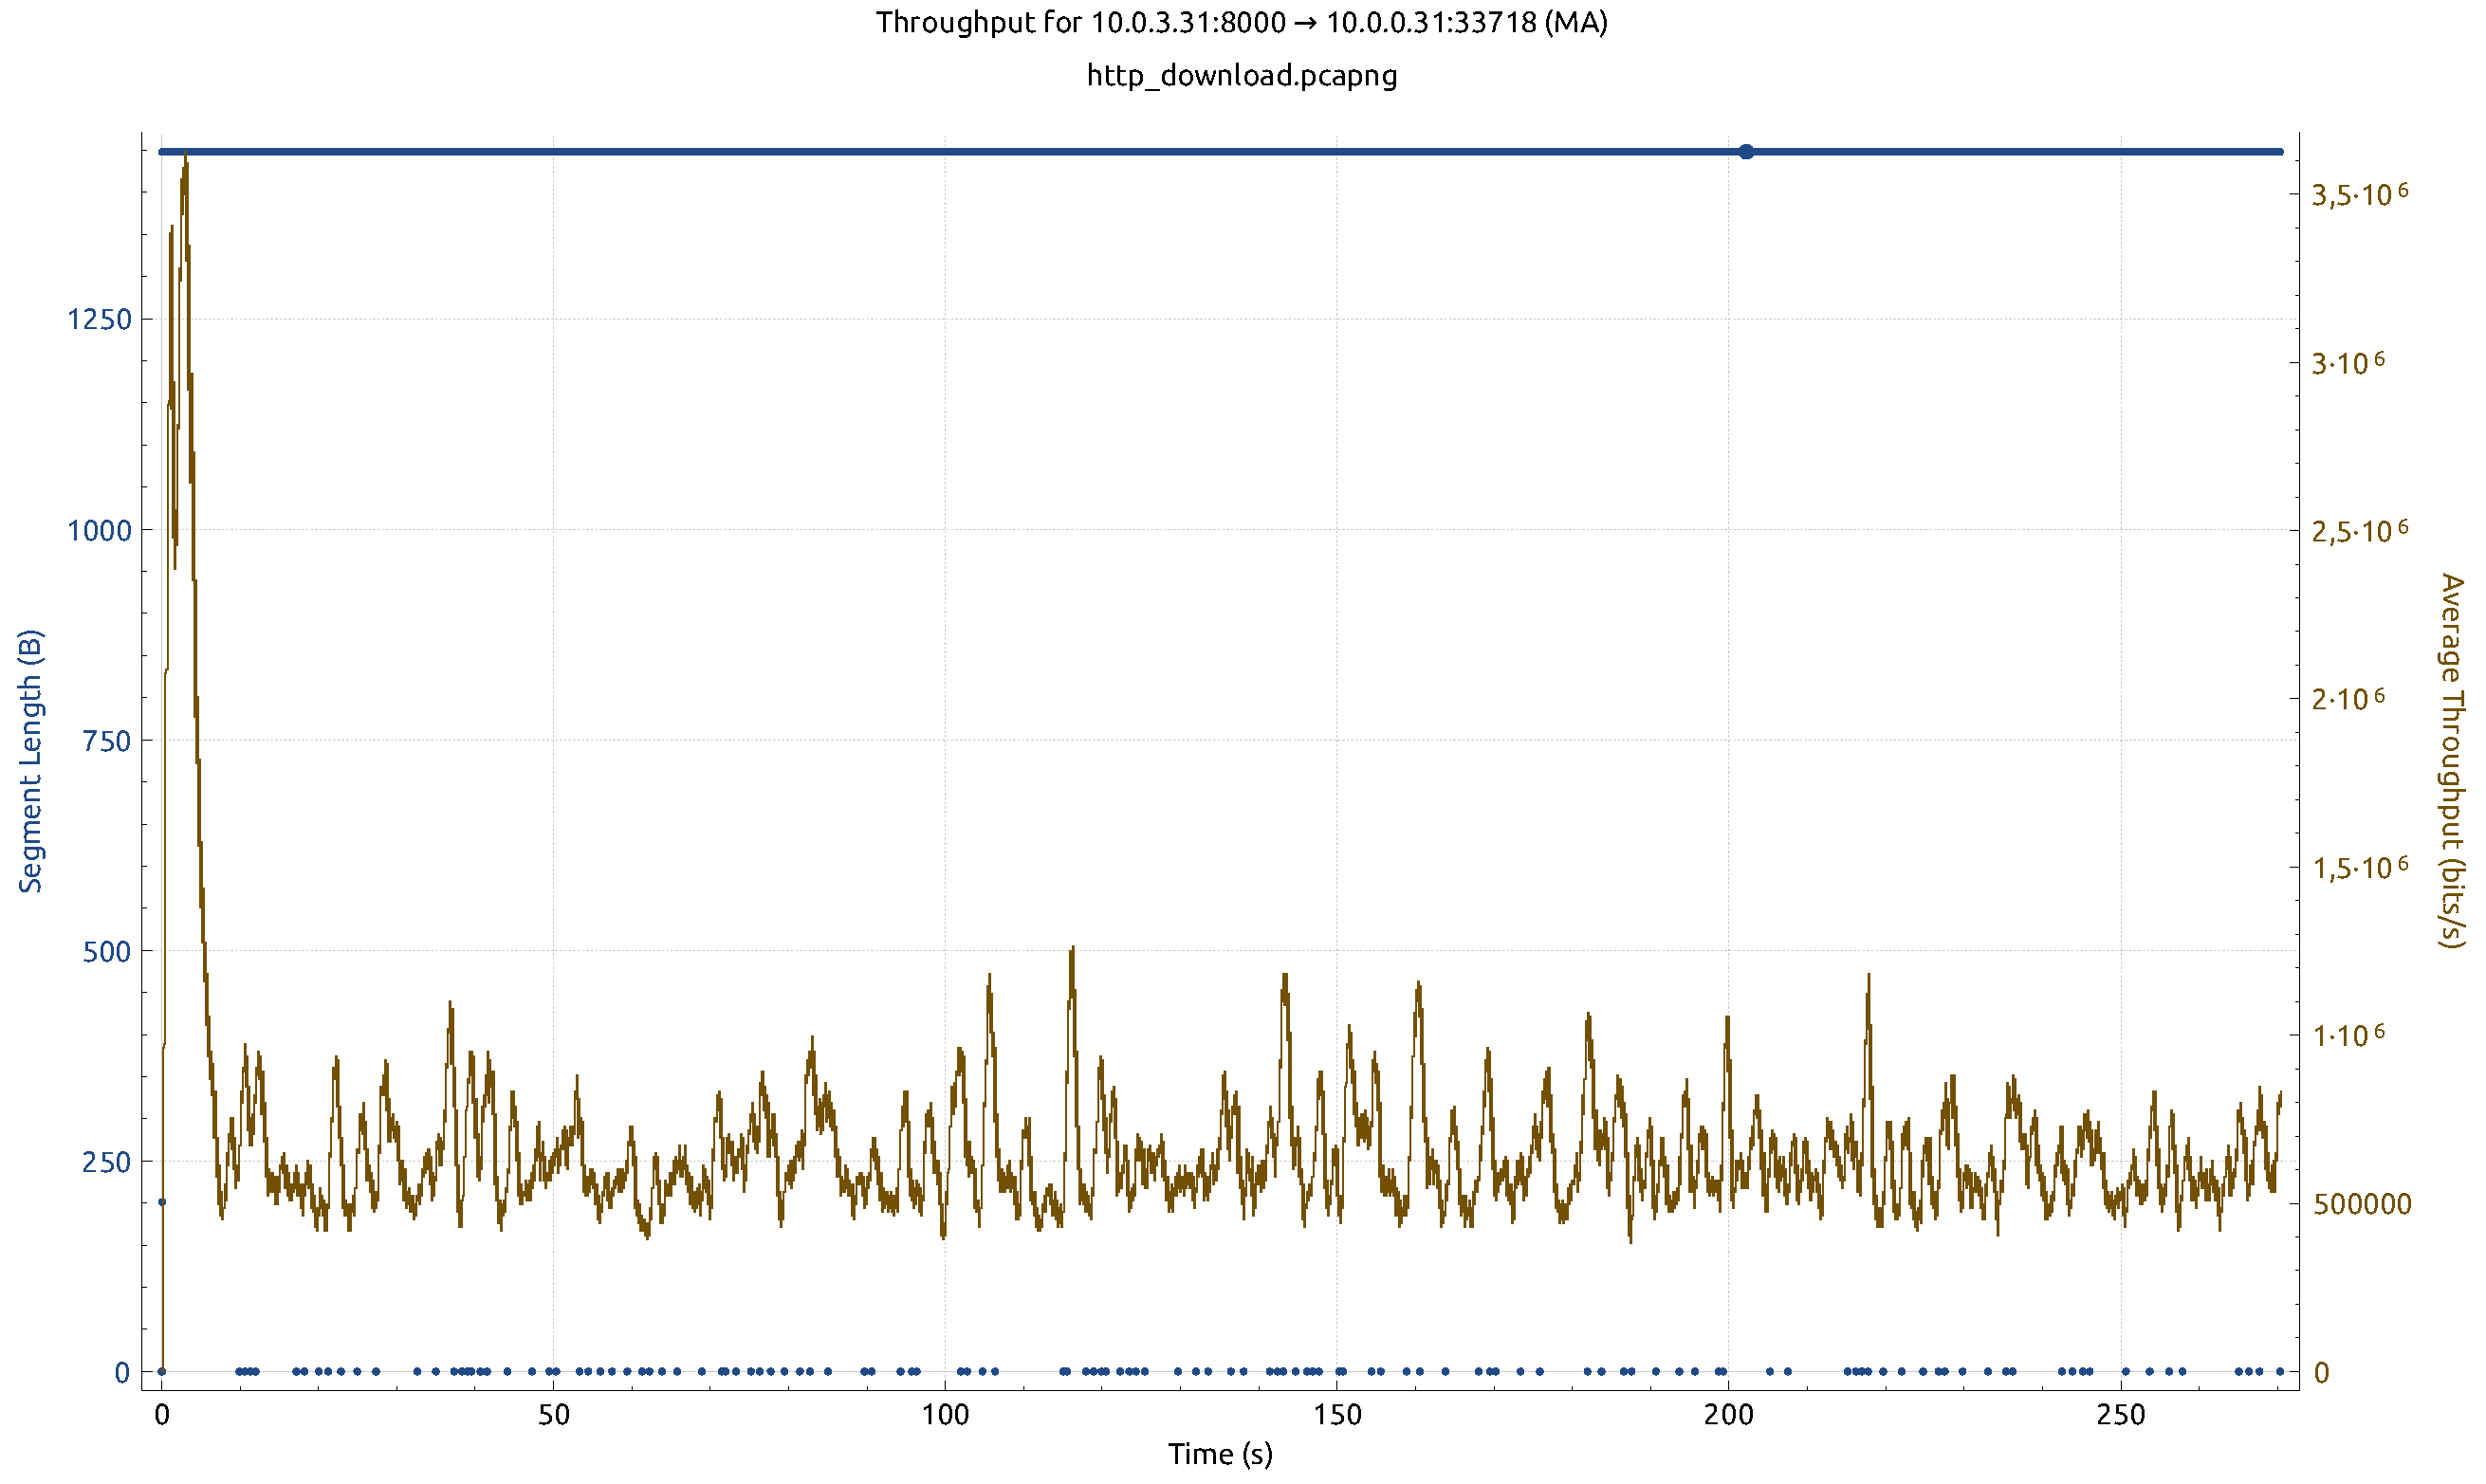
\includegraphics[height=0.66\textwidth,width=\textwidth]{fig/tcp_throughput.pdf}
        \caption{Throughput of a Duplicated Flow}
        \label{fig:dup_tcp}
\end{figure}

One of the unfortunate impacts of packet duplication is that it reduces the available bandwidth. It represents a waste of up to 50\% of the available resources, in the worst case, where every flow must be duplicated. Additionally, since flows which are being duplicated need to be re-ordered, this means that the FIFO approach for packets cannot be used and instead the packets must pass through a Packet Ordering and Elimination Function (POEF). When a packet arrives out of order the POEF starts to incur significant additional overhead because it must store all packets until the missing packet arrives, or a point is reached at which the stored packets must be dequeued. This point is either the point at which the packets expire, or the queue of out of order packets becomes full. Beyond this, the storing and eventual mass de-queuing of out of order packets can also interfere with the TCP algorithm- thus leading to reduced throughput.

These two effects - the POEF overhead and it's effects on TCP- lead to a very heavily reduced throughput, as can be seen in figure \ref{fig:dup:tcp}. The graph in the figure shows the throughput experienced by a routine TCP download, running over the WAN Connector, and experiencing replication, as well as the segment length of the TCP stream. As can be seen in the graph, the throughput is very low, and is not able to saturate the link's bandwidth despite being the only flow running at the time.

\section{Jitter Based Path Switching}

\begin{figure}[h]
    \centering
        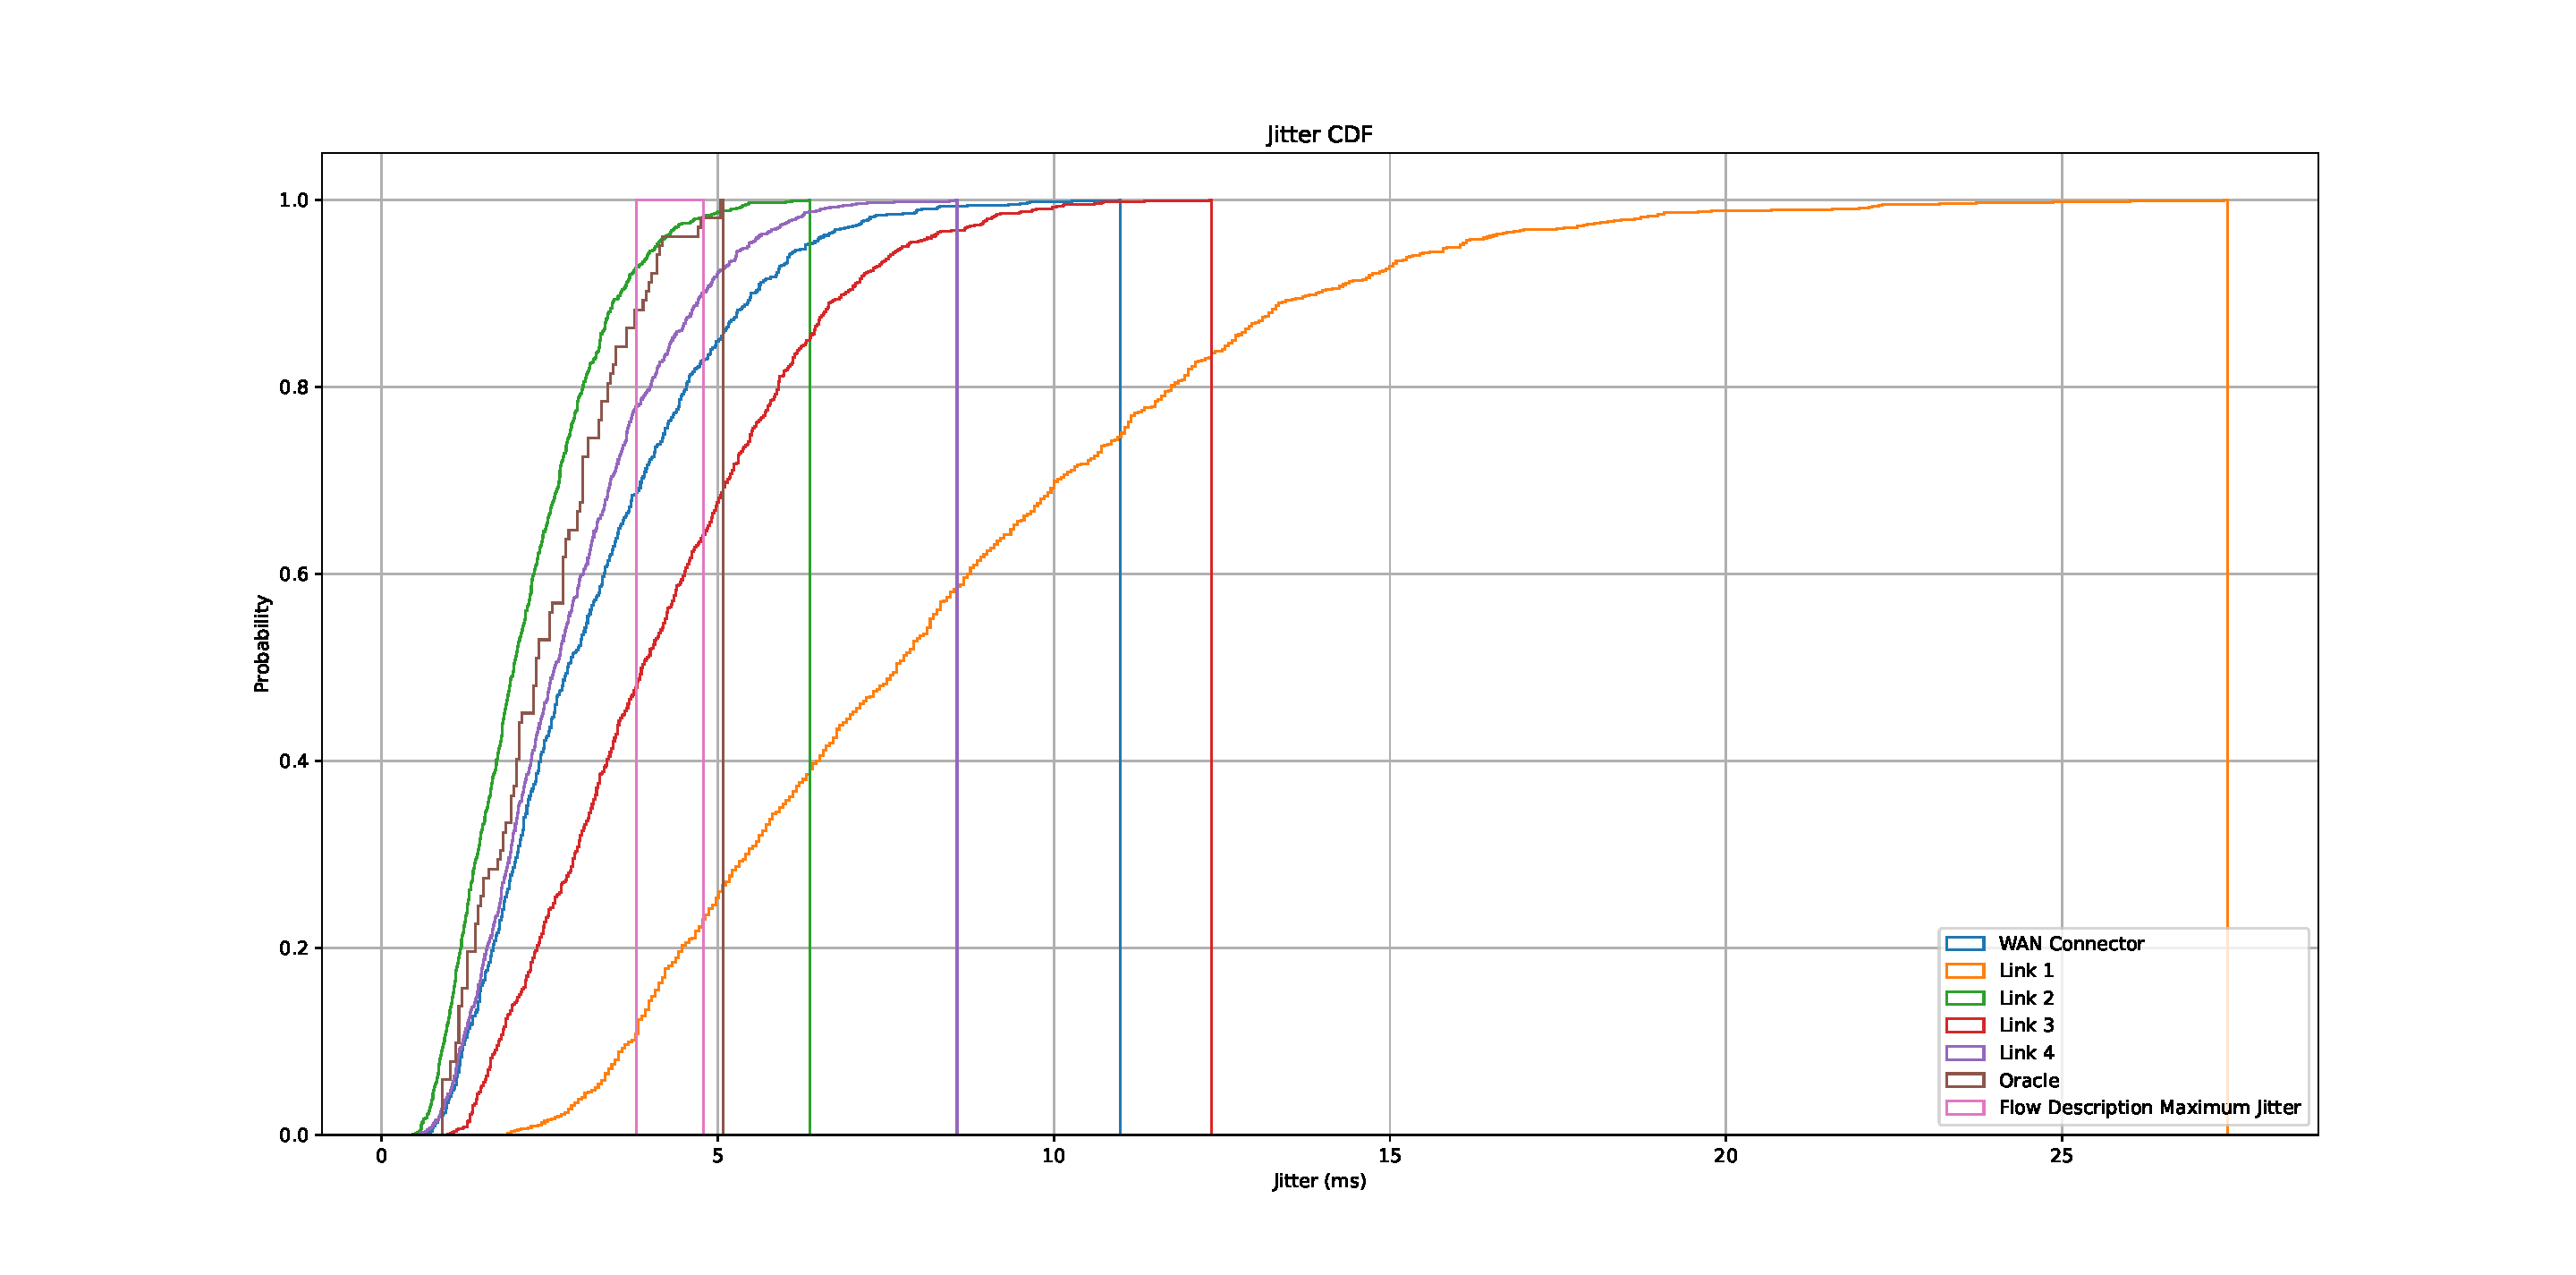
\includegraphics[height=0.66\textwidth,width=\textwidth]{fig/jitter_cdf.pdf}
        \caption{Performance of Jitter Based Path Switching}
        \label{fig:jitter_cdf}
\end{figure}

For the final analysis, the jitter must be investigated. For this purpose the simulation data was once again adapted. This time the standard deviation of the latency experienced was calculated for each of the 102 connections in the simulation. Then these standard deviations were scaled down by diving them by one, two, three, and four, respectively, in order to acquire four different set of jitter characteristics. Finally the scaled values were shuffled. This resulted in 4 links with varying jitter characteristics, which suffices for the emulation. Each different jitter value is emulated for 10 seconds on the respective link. During the emulation scenario a UDP iperf3 stream is ran at a rate of 3/4ths of the link's capability for 1000 seconds. iperf3 records jitter each second, and this data is used to then analyse the performance. Since more than half of the link capacity is being used by the flows being sent on the links (and not through the WAN Connector), the WAN Connector cannot be tested at the same time. Thus, to test the WAN Connector the emulation is repeated but with the flow only being sent over the WAN Connector. Lastly, the Oracle approach is calculated based on the simulation data. The Oracle approach, like before, displays the theoretical optimal performance. It chooses, at each point in time, the link with the lowest jitter. The cumulative distribution of the jitter experienced by the flows is plotted in figure \ref{fig:jitter_cdf}. 

As can be seen from the figure, the WAN Connector gave a very disappointing performance. It displays an inferior performance to two of the links. This means the path switching is actually causing a worse performance. This is most likely down to insufficient statistics causing poor path selection, because jitter statistics can't be gathered about other paths in this single flow scenario. The probe packets which are periodically sent out do not provide enough data points to accurately determine jitter. While they can give a sufficient baseline for latency calculations, as well as helping to determine if a link is dead or alive, their jitter measurements are not likely to provide a strong insight into the true nature of the link's jitter.

A final note about the plot in figure \ref{fig:jitter_cdf}. In the figure the first link actually performs better than the Oracle for most jitter values, before ultimately proving to have the greater maximum jitter values. This occurs because the Oracle is based on the simulation data and not the measurements. Therefore it is likely that the better performing link experienced, for the most part, very low jitter, and thus because there are more data points available than for the Oracle (and because no doubt there was some small amount of luck with the random values used by tc's netem qdisc), the percentage of packets below a certain level of jitter is greater. However ultimately the maximum values experienced by the flow, during those times when the link experiences it's worst jitter, are worse than the Oracle approach's worst cases, as one would expect.


\section{Discussion}

In light of these results one can conclude that the approach presented in the previous chapter is not without its flaws, however the results have also highlighted some of the functional aspects that were important for good performance. For latency based path switching it was able to outperform the other available links and achieve 80\% optimality, and the inclusion of a traffic shaper proved vital for preventing the latency critical flow from experiencing higher buffering times in the presence of a competing flow. For reliability, the WAN Connector showed that it was able to guarantee a critical flow a lower level of packet loss than would have been possible using any single link. Furthermore, it was even able to outperform the single link Oracle, and in a situation where the single link Oracle is unable to provide the required minimum level of packet loss for the desired flow, the WAN Connector was able to deliver the desired reliability. This is a hugely important result because it shows that the WAN Connector can provide greater reliability than even an optimal single link path selection algorithm, via the packet replication. This can enable critical applications to be run in environments where the backhaul options would usually be too unreliable to enable the critical applications.

This section, however, also demonstrates the downside of the packet replication approach, as it greatly reduces the overall throughput. Beyond this, during the jitter experiments, it is seen that the WAN Connector provides a poorer performance than simply using a single link for the entire experiment. This is fundamentally a bad result. The baseline by which any path selection algorithm should be judged is its ability to outperform the individual paths, since it can always select a superior option when one exists. Since the WAN Connector fails in this instance it must be concluded that it cannot provide an overall reduction in jitter for any jitter sensitive applications. The author would suggest, however, that the problem in this respect is not due to the design but rather the implementation. Ultimately there was not enough up to date information about the available links' jitter, so that the path selection algorithm could choose the right one.


%%=========================================
\section{Improvements}

There are several possible improvements that immediately spring to mind. These could be applied both to the actual implementation as well as to the high level design.

\subsubsection{Measuring and Predicting Path Characteristics}
Firstly, the path estimation could be adjusted to not just report previous statistics but also attempt to infer what the path might look like in the near future, for example as a path begins to experience increased latency a predictive algorithm/approach might be able to preemptively move flows off of that path, before their latency requirements are violated. This approach could be based on machine learning or AI, or it could use analytical methods.

Furthermore, it would be prudent to use an exponentially weighted averaging function when calculating a path's current characteristics, based on previous measurements. This would strike a nice balance between re-actively adjusting the predictions based on previous measurements and keeping in mind a path's performance across its entire history.

Also, as the authors in \cite{adaptive} did, this thesis' approach could benefit from adaptive windows of reporting. Instead of collecting statistics at a constant periodic rate, the rate can be adjusted to that period which performs best. This way there is not additional overhead with overly frequent statistical updates, as well as avoiding the reverse situation, where the reporting is too infrequent for a rapidly changing path.

Lastly, the probe packets which are sent out periodically to measure each path could be adjust to periodically be sent in large bursts, this would serve to provide a more accurate idea of the jitter and the packet loss, since these cannot be measured purely by sending a small number of probe packets. For accurate jitter and reliability measurements more packets are required. This may incur larger overhead on the link due to the bursts of extra packets, however one idea to counteract this would be to adjust the probing so that it is only performed on those links with insufficient traffic currently running through them. The links which are currently backhauling large amounts of traffic will be able to make their own measurements based purely on the backhaul traffic, and there may be no need at all for probe packets. Conversely, the underutilized links will not be able to make good estimations, and sending bursts of probe packets will not interfere with the actual traffic. This would present a solution to one of the biggest issues with the approach presented in this thesis.

\subsubsection{Adjustments for Jitter}

Another potential improvement would be to pass a "Time of Execution" field in the GTP header of packets of jitter-sensitive applications. This allows the receiving WAN connector to store packets if they have arrived too early, and, conversely, the packet ordering function may use this field to determine that it is more important to forward the current packet now, than to wait for a missing packet. This store and forward approach, with the time of execution field, is one of the solutions mentioned in the Deterministic Networking specification and would be a very sensible addition to this solution.

Additionally, specifically for the Lower Earth Orbit (LEO) satellite case, the path selection could potentially be adjusted to account for the periodic increases in latency as the current satellite leaves the range of the ground station, and the next one comes into range. For example during this phase it might make sense to temporarily forward packets on a different path, or to enable the store and forward mechanism, before disabling it once the satellite handover has passed.

\subsubsection{Forward Error Correction}

One possible improvement is the addition of Forward Error Correction (FEC). While this would be difficult to integrate into the equation to select paths, FEC could be used to increase the resilience of consistently lossy links, which is a big benefit for links which commonly exhibit this characteristic, such as wireless links. Especially LEO satellite links tend to present around 1\% packet loss \cite{deutschmann2022broadband}, which makes the use of FEC much more reasonable since one would only need to add a 2 to 5\% overhead, using a fountain code scheme, and thus wind up with a much more reliable link. However as was observed in the evaluation of the WAN Connector's throughput when using the Packet Ordering and Elimination Function, additional computation when receiving packets can lead to reduced overhead. To this extent, the addition of FEC would require efficient decoders and encoders on the sending and receiving side, so that the packet processing speed is not slowed down.

\subsubsection{Traffic Prioritization}

Perhaps the greatest theoretical flaw in the presented approach is that the WAN Connector does not perform packet prioritization, even though the 5G specifications explicitly mention that flows may have different priorities and should be prioritized accordingly. This is a significant flaw, and very difficult to account for. The most reasonable approach to integrating this is to add it to the traffic shaper. In the experiments performed here, the CAKE traffic shaper was used. It's implementation in the linux kernel does allow for up to 8 different priority 
"tins" for traffic, however that is not enough for the 5G requirements which allow for a great deal more priority levels than just 8. One option, therefore, would be to extend the CAKE implementation to allow a greater number of priority tins. Alternatively, the a different traffic shaper could be chosen, or developed, which incorporates prioritization as well as fairness and active queue management at the level of individual IP flows.


\subsubsection{Load Balancing}

In instances where more than one path is viable, the algorithm used for path selection does not account for the current load of the paths, nor does it try to perform load balancing when selecting paths. This is because the algorithm attempts to find the minimum weight path. Even in cases where two paths have the same properties and the same weighting, the algorithm does not attempt to shuffle or rotate between them. All flows with similar requirements will wind up on the same path. This can lead to under utilization of other paths and congestion problems on the "primary" path. This could be partially addressed by integrating a degree of random selection for equal paths. However a potentially more interesting approach would be to dynamically update the weights of different paths, based on their current load. This would keep randomness out of the algorithm, for reproducible results, and act as a form of load balancing. However great care would have to be taken with respect to how the weights are adjusted, so that paths are still appropriately weighted relative to each other. i.e. a path which is deemed twice as expensive as another path should not have more than half as much traffic as the other path, for flows which could go be forwarded on either path.















%!TEX root = ../thesis.tex

\cleardoublepage
\chapter{Conclusion and Outlook}
\label{cha:conclusion}

This thesis has looked at the use of reinforcement learning to size tasks in scientific workflows. It has provided definitions and a summary of scientific workflows, scientific workflow managers, the gradient bandit problem, and q-learning in the background chapter. It has discussed related work in chapter \ref{cha:related_work}, and then incorporated gradient bandits and q-learning into a popular workflow manager and tested their performance against the default configurations and a feedback-loop based approach. In the evaluation this thesis found that the results had vastly improved on the default configuration and had matched the feedback loop approach for performance while achieving greater CPU efficiency but worse memory efficiency.

This rest of this chapter briefly looks at what could be improved upon and what aspects may prove interesting for future research. Section \ref{sec:pot_improvements} considers what could be improved or done differently before section \ref{sec:implications} looks forwards and asks what implications this could have and what avenus might prove interesting for further research.

%%=========================================
\section{Potential Improvements}
\label{sec:pot_improvements}

Immediately the most obvious way in which these approaches could be improved upon would be to incorporate read and write calls into the reward function. When a thread reads or writes characters from or to a device it must perform a system call and wait for it to complete, and during this time the thread cannot use the CPU. If a program has a high degree of parallel operations but also has to read and write lots of characters then it would probably have lower CPU usage (because of the system calls) but simultaneously would benefit from being assigned more CPUs. However because of the nature of the bandit and the agent’s reward functions it is unlikely that this task would be assigned more resources since read and write calls are not considered.

Moving along this train of thought, it could also be prudent to incorporate the size of a task’s input file into the reward function for the memory bandit or the q-learning agent. A task’s memory footprint is most likely quite closely coupled with the size of the input file and this could prove important information for a reinforcement learning agent.

A different issue which was relevant to both approaches was the length of time needed to train the agents. The gradient bandit was trained for about 40 runs and the q-learning agent took 90 runs before they were “tested” across the next 10 runs. For large scale workflows this would take a considerable amount of time. Of course the agents are able to learn on the go and the performance during the training time is not so much worse as to make the workflows unusable during that time, so it is hard to say how much of a problem this could be.

Specifically for the q-learning agent there is room for improvement by incorporating replay buffers and eligibility traces. These would enable the agent to update its value function for the states and actions which led it to its current state and this is could help to learn an optimal $Q$ function faster. This is not done in the current implementation and could have a significant impact on performance. Additionally an epsilon of $\epsilon = 1/t$ could be used to decrease the agent’s exploration proportional to the time.

Finally, considering the testing set-up it would be an improvement to use kubernetes clusters with different machines to more accurately simulate the scenario where a workflow is performed on a larger distributed system with different nodes (with potentially heterogeneous resources). Such a set-up may also change results as the cumulative resources of the system would be greater, which may allows the agent’s decreased resource usage to increase throughput even more and thus speed up the workflows to a greater degree. It would also be better to use random inputs chosen from several different sets of possible inputs as opposed to repeating the workflows with the same input data. By training the agents using the same inputs there is a danger of overfitting the agents’ resource assignments. This may be less of a danger for the CPU assignments, because the character of a task’s CPU usage is less dependent on the size of the inputs, but repeatedly using the same inputs for an agent which sizes tasks for memory does present a real danger of overfitting. This is because the memory footprint of a task is much more dependent on the input to the task. This recommendation is not particularly relevant for those workflows which tend to have similarly sized inputs, but it could make a difference for workflows with different usage patterns.

%%=========================================
\section{Implications and Further Areas of Research}
\label{sec:implications}

The obvious implications of these findings are that, much like some of the scheduling problems mentioned in chapter \ref{cha:related_work}, this is also an area in which reinforcement learning has interesting potential. Additionally it has also shown that the resource configurations in scientific workflows have room for improvement and are another area which should be investigated further.

Nextflow and other scientific workflow managers represent a different class of actor in the interactions between user, application and execution platform. These workflow managers do not manage the execution platform, nor do they create the workflows which are executed. They are a kind of middle man and thus present a unique perspective on user-executor interactions. Normally the interactions in such environments are just between the user and the execution platform. The user has control over what process it wants to perform and how many resources to ask for, while the execution platform has control over when and how to execute the process. However in the context of a scientific workflow and a workflow manager, the manager sits in between the user and the execution platform and has no control over the tasks that must be executed nor over the execution. It is only capable of scheduling and sizing the tasks. This position requires a slightly different approach to common problems such as scheduling and resource assignment but it also presents an interesting avenue to research novel approaches to these familiar problems.

Now of the resources most important to both the process being executed and the user, the disk space must rank as one of the most important. Although it was not covered in this thesis, sizing a task’s disk space is another area where intelligent resource management could prove useful. It could most likely be solved in a fashion similar to the approach used for memory and in fact it would be quite simple to co-locate a gradient bandit approach for disk space alongside the memory and CPU bandits. Incorporating this into a q-learning agent would be trickier since the agent already has to explore a large state-action space for just memory and CPU, and by adding disk space into this it could become a very long process to try and train such an agent. Ultimately it may prove better to have separate q-learning agents for the CPU and the memory/disk-space (since these two are more likely to be closely related).

If one considers the current trends in machine learning and reinforcement learning agents then what could also be an interesting avenue for research would be to use deep reinforcement-learning \cite{deepQ}, which uses a deep neural network to learn a policy. This could allow for the kind of fine-grained memory assignments that made the feedback loop perform so well.

Following up on this idea, one more interesting area for further research would be incorporating a machine learning approach into a scientific workflow management systems’ internal scheduler. Whilst the reinforcement learning agents used in this thesis had no knowledge of the other tasks and of their interdependencies in the workflow, a scheduler would have the full understanding of a workflow’s digraph and could perhaps improve performance to an even greater degree by intelligently choosing when to assign a task slightly more or less resources than usual, depending on which tasks must wait for the current one to complete. 


% Include more chapters as required.

%%=========================================
%Backmatter

\appendix
%\include{backmatter/00_lessImportantText}
%\include{backmatter/01_acronyms}
%\include{backmatter/02_lexicon}
%%!TEX root = ../thesis.tex

\cleardoublepage
\chapter{Listings}
\label{app:listings}

This is the appendix for code, that does not need to be provided directly inside the thesis.

\section{Configuration for Node A}

%\lstinputlisting[style=json, caption={Configuration for Node A}, label={lst:nodeAConfig}]{listings/nodeAConfig.js}

%!TEX root = ../thesis.tex

\cleardoublepage
\chapter{Example of a Task’s Q-learning Agent}
\label{cha:qagent_example}

This appendix chapter contains a graphical representation of the q-learning agent for one of the tasks from the \textit{metaboigniter} workflow. The task was not chosen for any particular reason except that it only occurs once per workflow run and was thus only trained 100 times (other tasks occur multiple times within the same workflow and are thus trained more often). 

\begin{figure}[ht]
    \centering
	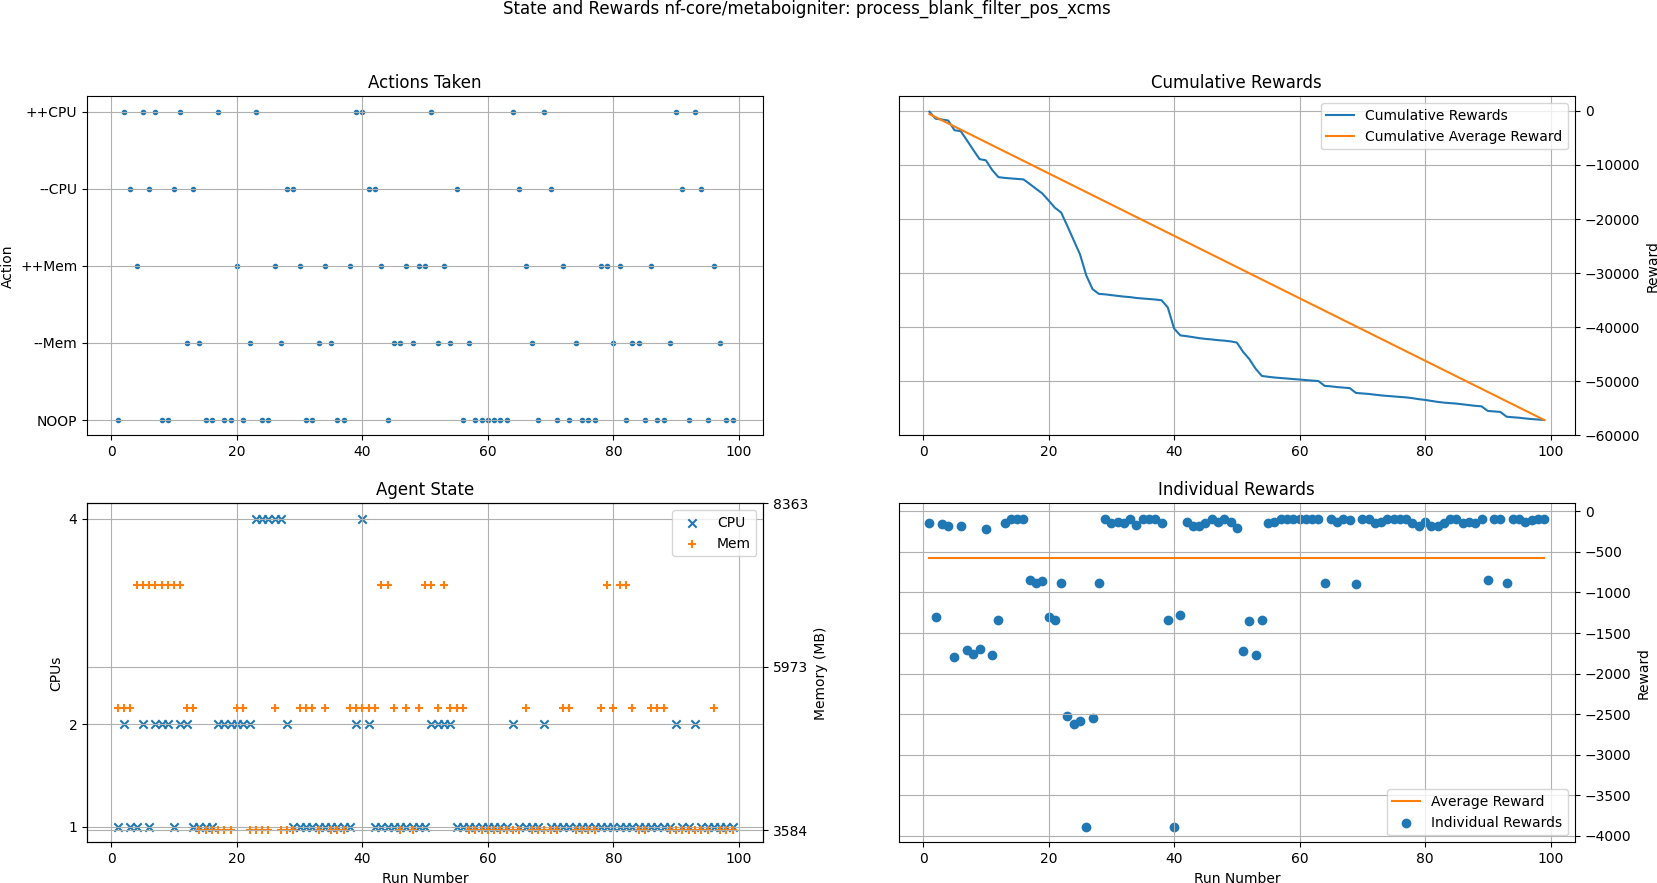
\includegraphics[width=\textwidth]{fig/qagent_cropped.png}
	\caption{Example of a Q-learning Agent}
	\label{fig:q_example}
\end{figure}

There are 4 graphs in \ref{fig:q_example} the top left graph is a scatter plot which indicates what action the agent took at what point in time. The bottom left graph indicates what the agent’s CPU and memory allocation (its state) was at that point in time. Meanwhile the top right graph shows the agent’s cumulative rewards over time, as well as a straight line which represents what the cumulative reward would look like if the reward was consistent. It should be noted that because the reward function is negative, whenever the line’s slope is steep the agent is performing poorly and receiving low rewards, whilst near-horizontal slopes show that the agent is doing well and limiting its punishment (receiving higher rewards). Finally the bottom right graph is a simple scatter plot of what rewards the agent received, with a constant line to show the average reward.

This figure is useful both to indicate that the agent is actually trying to learn favourable actions, as well as to represent what states the agent is exploring. 

% Include more appendices as required.

\cleardoublepage
\addcontentsline{toc}{chapter}{Bibliography}
\printbibliography[heading=bibliography]
%\defbibheading{notonline}{\chapter*{Bibliography}}
%\printbibliography[heading=notonline, nottype=online]
%\defbibheading{online}{\chapter*{Bibliography (Online)}}
%\printbibliography[heading=online, type=online]

%%=============================================

\end{document}
